\documentclass[a4paper,10pt]{ltjsarticle}
\usepackage[margin=22mm]{geometry}
\usepackage{booktabs}
\usepackage{array}
\newcolumntype{L}[1]{>{\raggedright\arraybackslash}p{#1}}
\usepackage{graphicx}
\usepackage{amsmath,amssymb}
\usepackage{caption}
\usepackage{subcaption}
\usepackage{float}
\usepackage{adjustbox}
\usepackage{tikz}
\usetikzlibrary{arrows.meta,positioning,patterns,calc,decorations.pathreplacing}
\usepackage{pgfplots}
\pgfplotsset{compat=1.18}
\usepackage[most]{tcolorbox}
\usepackage{listings}
\lstset{language=Python, basicstyle=\ttfamily\scriptsize, keywordstyle=\bfseries,
  commentstyle=\itshape\color{black!70}, stringstyle=\ttfamily, columns=fullflexible, keepspaces=true,
  frame=tb, framerule=0.4pt, breaklines=true, showstringspaces=false, aboveskip=6pt, belowskip=4pt,
  captionpos=t, xleftmargin=2pt}
\renewcommand{\lstlistingname}{コード}
\usepackage[hidelinks]{hyperref}
\graphicspath{{figures/}}

% monochrome emphasis box
\newtcolorbox{keybox}[1]{enhanced, colback=white, colframe=black, boxrule=0.6pt, arc=0pt,
  left=6pt, right=6pt, top=4pt, bottom=4pt, fonttitle=\bfseries, coltitle=black,
  colbacktitle=black!12, title={#1}}

\title{Gemma 4 のサービング性能\\[2pt]
\large H100 NVL 1 基 / vLLM 0.32 での TTFT・Decode・MTP Drafter の実測と理論限界}
\author{}
\date{2026年10月}

\begin{document}
\maketitle

\begin{abstract}
Gemma~4 ファミリ（E2B, E4B, 12B, 26B-A4B MoE, 31B Dense）を NVIDIA H100~NVL 1 基上の vLLM 0.32.0 で
OpenAI 互換サーバとして動かし，TTFT，TPOT，同時実行時のスループット，および公式 MTP Drafter によるspeculative decodingの効果を測定した．
比較対象は Qwen3-30B-A3B と Qwen3-32B である．
測定値はチェックポイントから計算したroofline上の理論限界と突き合わせた．
大きい dense モデルの decode は HBM 帯域の 70\% に達し，MTP で最大 3.1 倍速くなる．
長いコンテキストの decode は vLLM 0.32.0 では Qwen3 より遅いが，原因は FlashAttention-4 カーネルの split-KV のバグ（128 個の CTA のうち 1 個しか働かない）であり，
1 行の修正で 30k トークンでの TPOT は最大 4.6 倍速くなり，Qwen3 を上回る．
一方，高並列での KV キャッシュ容量とスループットでは，Hybrid Attentionのアーキテクチャ上の利点を現状の vLLM が活かしきれていない．
\end{abstract}

\tableofcontents
\newpage

%=====================================================================
\section{Gemma 4 とは}
\label{sec:gemma4}
Gemma~4 は Google DeepMind が 2026 年に公開したオープンウェイトのモデルファミリである\cite{gemma4tr,gemma4card,hfblog}．
端末向けの E2B / E4B から，GPU 1 基で動く 12B・26B-A4B（MoE）・31B（dense）まで 5 サイズがある（図\ref{fig:family}）．
2026 年 5 月には，speculative decoding用の小型モデル \textbf{MTP Drafter} が全サイズ向けに追加公開された\cite{gemma4x,mtpblog}．

\begin{figure}[htbp]\centering
\begin{adjustbox}{max width=\linewidth}% Gemma 4 family: total text parameters vs. parameters read per decoded token
\begin{tikzpicture}
\begin{axis}[
  xbar, bar width=7pt, width=0.82\linewidth, height=5.2cm,
  xmin=0, xmax=36, xlabel={パラメータ数 [B]},
  symbolic y coords={31B,26B-A4B,12B,E4B,E2B}, ytick=data, y dir=reverse,
  yticklabel style={font=\small},
  enlarge y limits=0.15, axis x line*=bottom, axis y line*=left,
  legend style={draw=none, at={(0.98,0.04)}, anchor=south east, font=\footnotesize, cells={anchor=west}},
  nodes near coords align={horizontal},
]
% total (text tower) parameters, hollow
\addplot+[bar shift=0pt, draw=black, fill=white, pattern=north east lines,
          nodes near coords={\pgfmathprintnumber[fixed,precision=1]{\pgfplotspointmeta}},
          every node near coord/.append style={font=\scriptsize, black}]
  coordinates {(4.6,E2B) (7.5,E4B) (11.9,12B) (25.2,26B-A4B) (30.7,31B)};
% parameters touched per token in decode, solid
\addplot+[bar shift=0pt, draw=black, fill=black!75]
  coordinates {(2.3,E2B) (4.7,E4B) (11.9,12B) (3.8,26B-A4B) (30.7,31B)};
\legend{総パラメータ（テキスト部）, 1 トークンの decode で読むパラメータ}
\end{axis}
\end{tikzpicture}
\end{adjustbox}
\caption{Gemma 4 ファミリ．E2B/E4B は総パラメータの約半分が層ごとのembeddingテーブル（PLE）で，26B-A4B は MoE である．
どちらも 1 トークンの decode で実際に読むパラメータは総数よりずっと少ない（数値は本書で測ったチェックポイントの値）．}
\label{fig:family}
\end{figure}

Gemma~4 には，同じ性能をより少ない計算量とメモリで出すための工夫が多い．
\begin{itemize}
\item \textbf{Hybrid Attentionと K=V}：大半の層を sliding window Attentionにして，長いコンテキストでの KV キャッシュを減らす．global 層では value を key と同じprojectionから作る（V projectionの重みを持たない）．
\item \textbf{KV 共有と PLE}（E2B/E4B）：後段の層が前段の KV を再利用する．巨大なembeddingテーブルは lookup だけで済ませる．
\item \textbf{MoE}（26B-A4B）：1 トークンで使う重みを総 25B のうち 3.8B に絞る．
\item \textbf{MTP Drafter}：小型の drafter が次の数トークンを予測し，本体が 1 回の forward でまとめてverifyする．
\end{itemize}
いずれも，サービスとして動かしたときの応答開始までの時間，生成速度，同時に処理できるリクエスト数に直接効くはずの設計である．
ただし，その効果が実際の推論エンジン上でどれだけ表れるかは，公式資料だけでは分からない．

\begin{keybox}{本書の目的}
Gemma~4 の\textbf{サービング性能}を，同じ GPU・同じ推論エンジン（H100~NVL 1 基，vLLM 0.32）の上で測り，
同クラスの Qwen3（30B-A3B MoE / 32B dense）と比較する．
測定値はすべてチェックポイントから計算した理論限界と突き合わせ，
\textbf{どこまで性能を出し切れているか}と\textbf{何が律速しているか}を数値で示す．
\end{keybox}

%=====================================================================
\section{はじめに}
モデルカードが報告するのは主に精度であり，推論速度は GPU と推論エンジンの組み合わせで大きく変わる．
本書では Gemma~4 の設計上の工夫が，実際のサービング性能にどう表れるかを次の 4 つの問いで調べる．
\begin{description}
\item[Q1] Gemma~4 は GPU の性能（HBM 帯域・演算性能）をどこまで出し切れているか．
\item[Q2] Hybrid Attention・K=V・MoE は，同クラスの Qwen3 に対して実際に速さや容量の差を生むか．
\item[Q3] MTP Drafter はどの条件でどれだけ速くなるか．効果の差は何で決まるか．
\item[Q4] 理論値に届かない場合，何が律速しているか．
\end{description}

\paragraph{主な結果．}
\begin{enumerate}
\item 31B の decode は HBM 理論帯域の 70\% に達し，ほぼ理論どおりに動く．小さいモデルと MoE は 28--38\% にとどまる．
      Nsight Systems で分解すると，重みの読み出し以外にかかる時間（SM を埋めきれない小さな GEMM，normalizationなどの小さなカーネル群，Attention，GPU idle）は
      モデルの大きさによらず 1 ステップ 2.7--4.6\,ms あり，読むバイトが少ない小さいモデルほどこの一定の上乗せが相対的に重くなるためである（\S\ref{sec:short}）．
\item Hybrid Attentionは長いプロンプトの prefill で効き，32k トークンの TTFT は Qwen3 より 16--33\% 短い．
      sliding window でAttentionの FLOPs が減るためで，その差はAttentionが FLOPs の大きな割合を占める 4k トークン以上で現れ，window size（1024）以下では差がない（\S\ref{sec:prefill}）．
      一方，vLLM 0.32.0 では長いコンテキストの decode が，KV の読み出し量が Qwen3 の 3--4 割しかないのに Qwen3 より遅い．
      プロファイルでは，global 層のAttentionカーネルが理論どおりのバイト数しか読んでいないのに HBM 帯域の 1\% 未満しか使っていない．
      原因は FA4 カーネルの split-KV に分割数が渡っていないバグで，128 個の CTA のうち 1 個だけがすべての KV を読んでいた（\S\ref{sec:ctx}）．
      1 行の修正で 30k での TPOT は E2B で 17.0\,ms から 3.7\,ms，31B で 40.7\,ms から 23.3\,ms になり，31B は Qwen3-32B（24.9\,ms）より速くなる（\S\ref{sec:ctx-fix}）．
      この修正は upstream にすでに入っており，v0.32.1rc0 以降で使える．
\item MTP Drafter は単一ストリームの decode を 1.35--3.1 倍速くする．効果は 31B で最大，26B-A4B で最小であり，この差は帯域のコストモデルで説明できる．
\item 短いリクエストを高並列で処理すると，31B は 64 並列で Qwen3-32B の 0.6 倍のスループットしか出ない．KV キャッシュが足りずリクエストが待たされるが，FP8 KV キャッシュで KV 容量を 1.9 倍にしても待ち時間が減るだけでスループットは変わらない（\S\ref{sec:conc}）．
\end{enumerate}

\paragraph{本書の構成．}
\S\ref{sec:framework} で分析に使う枠組み（rooflineモデルとspeculative decodingのコストモデル）と計測ツールを導入し，
\S\ref{sec:env} で実験環境のハードウェア性能を示す．
\S\ref{sec:arch} で Gemma~4 のアーキテクチャを推論性能の観点から整理し，\S\ref{sec:theory} でそれを理論限界の式に落とす．
\S\ref{sec:method} で実験方法を述べ，\S\ref{sec:results} で結果を示す．
\S\ref{sec:discussion} では外部の結果と比べたうえで，Qwen3 に対して良い結果だったのか，コミュニティとして何をすべきかを論じ，\S\ref{sec:tuning} でボトルネックと対策をまとめる．

%=====================================================================
\section{性能分析の枠組み}
\label{sec:framework}

\subsection{Prefill と Decode}
LLM の推論 1 リクエストは，プロンプトを一括処理する \textbf{prefill} と，1 トークンずつ生成する \textbf{decode} に分かれる（図\ref{fig:pd}）\cite{kotoba}．
本書では次の 3 つの指標を使う．
\begin{itemize}
\item \textbf{TTFT}（Time To First Token）：リクエストを送ってから最初のトークンが返るまでの時間．主に prefill で決まる．
\item \textbf{TPOT}（Time Per Output Token）：2 トークン目以降の 1 トークンあたりの生成時間．decode 1 ステップの時間に等しい．
\item \textbf{スループット}：全リクエスト合計の出力トークン数 / 秒．同時実行数を増やすと上がる．
\end{itemize}

\begin{figure}[htbp]\centering
\begin{adjustbox}{max width=\linewidth}% One request: prefill (all prompt tokens at once) then token-by-token decode
\begin{tikzpicture}[x=1cm, y=1cm, font=\small,
  blk/.style={draw, minimum height=0.8cm, inner sep=1pt, align=center}]
% time axis
\draw[-{Stealth}] (0,0) -- (14.6,0) node[right] {時刻};
\node[below, font=\scriptsize] at (0,0) {要求到着};
% prefill block
\node[blk, fill=black!20, minimum width=4.2cm, anchor=south west] (pf) at (0,0.25)
  {\textbf{Prefill}\\[-1pt]\scriptsize プロンプト $P$ トークンを一括処理};
% decode steps
\foreach \i in {0,...,5} {
  \node[blk, fill=white, minimum width=1.2cm, anchor=south west] (d\i) at ({4.4+1.4*\i},0.25)
    {\scriptsize step\,\pgfmathparse{int(\i+1)}\pgfmathresult};
}
\node[font=\small] at (13.3,0.65) {$\cdots$};
% output tokens
\foreach \i in {0,...,5} {
  \draw[-{Stealth}] ({4.4+1.4*\i+0.6},1.05) -- ++(0,0.45) node[above, font=\scriptsize] {$y_{\pgfmathparse{int(\i+1)}\pgfmathresult}$};
}
% TTFT and TPOT braces
\draw[decorate, decoration={brace, mirror, amplitude=4pt}] (0,-0.45) -- (4.4,-0.45)
  node[midway, below=4pt] {TTFT};
\draw[decorate, decoration={brace, mirror, amplitude=4pt}] (5.0,-0.45) -- (6.4,-0.45)
  node[midway, below=4pt] {TPOT};
% characteristics
\node[align=left, font=\scriptsize, anchor=north west, text width=4.2cm] at (0,-1.25)
  {重みを 1 回読んで $P$ トークン分を計算\\ $\Rightarrow$ arithmetic intensity $\approx P$：\textbf{計算律速}};
\node[align=left, font=\scriptsize, anchor=north west] at (4.4,-1.25)
  {1 step ごとに全重み＋KV キャッシュを読んで $B$ トークン分を計算（$B$：同時実行数）\\
   $\Rightarrow$ arithmetic intensity $\approx B$：$B$ が小さいと\textbf{メモリ帯域律速}};
\end{tikzpicture}
\end{adjustbox}
\caption{1 リクエストの処理の流れ．prefill と decode では律速要因が異なる．}
\label{fig:pd}
\end{figure}

\subsection{rooflineモデル}
\label{sec:roofline}
ある処理が $F$ [FLOP] の演算と $Q$ [byte] のメモリ転送を必要とするとき，
演算ピーク $\pi$ [FLOP/s]，メモリ帯域 $\beta$ [byte/s] の GPU での実行時間は
\begin{equation}
t \;\ge\; \max\!\left(\frac{F}{\pi},\ \frac{Q}{\beta}\right)
\label{eq:roofline}
\end{equation}
で下から抑えられる．演算と転送が完全に重なった理想的な状態でも，どちらか遅い方より速くはならないからである．
両辺を $F$ で割ると，到達できる演算性能は $F/t \le \min(\pi,\ I\beta)$ となる．ここで $I = F/Q$ を\textbf{arithmetic intensity}（1 byte 転送あたりの演算量）と呼ぶ．
これを図にしたものがroofline（図\ref{fig:roofline-concept}）で，折れ曲がる点
\begin{equation}
I^\ast = \pi / \beta
\end{equation}
を\textbf{ridge point}と呼ぶ．$I < I^\ast$ ならメモリ帯域律速，$I > I^\ast$ なら計算律速である．
式\eqref{eq:roofline}はキャッシュ，カーネル起動，CPU 側の処理を無視した下限なので，
\textbf{実測値と下限の差}が「その他の要因」による損失，つまり改善の余地を表す．

\paragraph{LLM への適用．}
BF16 の重みは 1 パラメータ 2\,byte で，1 トークンの計算では各パラメータを 1 回の積和（2\,FLOP）に使う．
decode で $B$ 本の系列を 1 ステップ進めるとき，重みは $B$ 本で共有して 1 回だけ読めばよいので，
$F \approx 2NB$，$Q \approx 2N$（$N$ はパラメータ数）となり，$I \approx B$ である．
同様に，$P$ トークンの prefill では $I \approx P$ になる．
この関係は LLM 推論の性能分析でよく使われるもので，文献\cite{kotoba} は「バッチサイズ＝合計トークン数と考えるとシンプル」と述べ，
文献\cite{kipply} は A100 では同じ議論から「バッチサイズ 208 未満の decode はメモリ帯域律速」と見積もっている．
ここでの $I \approx B$ は重みの読み出しだけを数えた近似であり，KV キャッシュは系列ごとに別に読むので，コンテキストが長いと実際の $I$ はこれより小さい．
したがって decode は同時実行数 $B$ が $I^\ast$ を超えるまでメモリ帯域律速で，prefill は数百トークン以上で計算律速になる．

\begin{figure}[htbp]\centering
\begin{adjustbox}{max width=\linewidth}% Roofline of H100 NVL (datasheet and measured) with typical operating points
\begin{tikzpicture}
\begin{loglogaxis}[
  width=0.72\linewidth, height=6.2cm,
  xmin=0.5, xmax=20000, ymin=1, ymax=2000,
  xlabel={arithmetic intensity $I$ [FLOP/byte]}, ylabel={到達性能 [TFLOPS]},
  log basis x=10, log basis y=10, grid=major, grid style={black!12},
  axis x line*=bottom, axis y line*=left, font=\small,
  legend style={draw=none, fill=none, at={(0.5,-0.22)}, anchor=north, font=\scriptsize, cells={anchor=west}}, legend columns=2,
]
% datasheet roof: min(3.9 TB/s * I, 835 TFLOPS)
\addplot[black, thick, domain=0.5:20000, samples=200] {min(3.9*x, 835)};
% measured roof: min(3.57 TB/s * I, 492 TFLOPS)
\addplot[black, dashed, domain=0.5:20000, samples=200] {min(3.57*x, 492)};
\legend{{データシート（3.9\,TB/s，835\,TFLOPS）}, {本機の実測（3.57\,TB/s，492\,TFLOPS）}}
% ridge point
\draw[densely dotted] (axis cs:214,1) -- (axis cs:214,835);
\node[font=\scriptsize, anchor=west] at (axis cs:230,1.6) {$I^\ast\!=\!214$};
% operating points
\addplot[only marks, mark=*, mark size=2pt] coordinates {(1,3.9)};
\node[font=\scriptsize, anchor=west] at (axis cs:1.15,3.0) {decode $B{=}1$};
\addplot[only marks, mark=*, mark size=2pt] coordinates {(64,249.6)};
\node[font=\scriptsize, anchor=west] at (axis cs:70,190) {decode $B{=}64$};
\addplot[only marks, mark=square*, mark size=2pt] coordinates {(4096,835)};
\node[font=\scriptsize, anchor=north] at (axis cs:4096,330) {prefill $P{=}4\text{k}$};
% region labels
\node[font=\scriptsize, rotate=0, anchor=west] at (axis cs:0.7,40) {\textbf{メモリ帯域律速}};
\node[font=\scriptsize, anchor=south] at (axis cs:2500,1050) {\textbf{計算律速}};
\end{loglogaxis}
\end{tikzpicture}
\end{adjustbox}
\caption{本機（H100 NVL）のrooflineと典型的な動作点．decode のarithmetic intensityはバッチサイズ $B$，prefill はプロンプト長 $P$ にほぼ等しい．}
\label{fig:roofline-concept}
\end{figure}

\subsection{speculative decodingのコストモデル}
\label{sec:specmodel}
speculative decodingでは，軽い drafter が $\gamma$ トークンを順に予測し，
本体（target）が $\gamma+1$ 位置を 1 回の forward でまとめてverifyする（図\ref{fig:specdec}）．
先頭から一致したトークンと，target 自身が出す 1 トークンが確定する．
1 回のverifyで確定するトークン数の平均を\textbf{mean acceptance length} AL（$1 \le \mathrm{AL} \le \gamma+1$）とする．
greedy 生成なら出力は通常の decode と完全に一致する．

1 回のspeculative step（drafter $\gamma$ 回＋verify 1 回）の時間が通常の decode 1 ステップの $c$ 倍だとすると，
$c$ ステップ分の時間で AL トークンが確定するので，
\begin{equation}
\text{TPOT 高速化} = \frac{\text{TPOT}_\text{base}}{\text{TPOT}_\text{spec}} = \frac{\mathrm{AL}}{c}
\label{eq:spec}
\end{equation}
となる．AL は drafter の予測精度，つまり生成内容で決まる．$c$ は drafter とverifyの\emph{コスト}で，モデル構造とハードウェアで決まる．
両者を分けて測れば，「acceptance rateが低いから遅い」のか「verifyが高くつくから遅い」のかを区別できる．
$c$ の理論値は \S\ref{sec:theory-spec} で導く．

\begin{figure}[htbp]\centering
\begin{adjustbox}{max width=\linewidth}% Plain decode vs. speculative decode (gamma = 4)
\begin{tikzpicture}[x=1cm, y=1cm, font=\small,
  tgt/.style={draw, fill=black!25, minimum height=0.6cm, minimum width=1.6cm, inner sep=0pt, align=center},
  drf/.style={draw, fill=white, minimum height=0.6cm, minimum width=0.35cm, inner sep=0pt}]
% plain decode
\node[anchor=east, align=right] at (-0.2,1.6) {通常の decode};
\foreach \i in {0,...,3} {
  \node[tgt, anchor=west] at ({1.7*\i},1.6) {\scriptsize target};
  \node[font=\scriptsize] at ({1.7*\i+0.8},2.15) {+1 token};
}
% speculative decode
\node[anchor=east, align=right] at (-0.2,0.2) {speculative decoding\\[-2pt]\scriptsize ($\gamma=4$)};
\foreach \j in {0,1,2,3} { \node[drf, anchor=west] at ({0.4*\j},0.2) {}; }
\node[font=\scriptsize] at (0.8,-0.35) {draft $\times\gamma$};
\node[tgt, anchor=west, minimum width=1.9cm] (v) at (1.65,0.2) {\scriptsize verify $\gamma{+}1$};
\node[font=\scriptsize, align=center] at (2.6,0.85) {AL token 確定};
\draw[decorate, decoration={brace, mirror, amplitude=4pt}] (0,-0.65) -- (3.55,-0.65)
  node[midway, below=4pt, font=\scriptsize] {1 speculative step $=$ 通常 step の $c$ 倍の時間};
% legend
\node[tgt, minimum width=0.6cm, anchor=west] at (8.0,1.0) {};
\node[anchor=west, font=\scriptsize] at (8.65,1.0) {target（本体）の forward};
\node[drf, anchor=west] at (8.12,0.3) {};
\node[anchor=west, font=\scriptsize] at (8.65,0.3) {drafter の forward（軽い）};
\node[anchor=west, font=\small] at (8.0,-0.5) {TPOT 高速化 $= \mathrm{AL}/c$};
\end{tikzpicture}
\end{adjustbox}
\caption{通常の decode とspeculative decoding．speculative step 1 回で平均 AL トークンが確定し，時間は通常の $c$ 倍かかる．}
\label{fig:specdec}
\end{figure}

\subsection{GPU の実行モデル：SM・CTA・wave と latency}
\label{sec:gpu-model}
ルーフラインは「十分な並列度がある」ことを前提にした上限である．
実測が上限から遠いとき，その原因を調べるには GPU がカーネルをどう実行するかを知っておく必要がある\cite{nvperf,cudaguide}．

\paragraph{SM と CTA．}
H100 NVL は 132 個の \textbf{SM}（Streaming Multiprocessor）を持つ\cite{h100wp}．
カーネルは \textbf{CTA}（Cooperative Thread Array，CUDA では thread block）の集まり（grid）として起動され，1 つの CTA は 1 つの SM 上で実行される．
CTA は 32 thread ずつの \textbf{warp} に分かれ，SM は最大 64 warp（2048 thread）を同時に抱えて，待ちの発生した warp から別の warp に切り替えながら実行する．
同時に実行される CTA の一群を \textbf{wave} と呼ぶ．NVIDIA は，CTA の数を SM の数の数倍以上にして複数の wave で実行するのが効率的だとしている\cite{nvperf}．
CTA が SM より少ないと，仕事のない SM が生じ，その SM の演算器もメモリ帯域も使われない（図\ref{fig:smfill}(a)）．

\paragraph{latency hiding と Little の法則．}
HBM からのロードには数百 ns かかる．この待ち時間（latency）の間も帯域を埋めるには，常に大量のロードを発行中にしておく必要がある．
Little の法則によれば，到達できる帯域は「発行中のバイト数 / latency」で決まる\cite{volkov}．
仮に latency を 500\,ns とすると，3.9\,TB/s を出すには約 2\,MB，SM 1 個あたり十数 KB のロードを常に発行中にしておかなければならない．
SM 上の warp が少ない（occupancy が低い）か，1 warp が逐次にしかロードを出さないと，この条件を満たせない（図\ref{fig:smfill}(b)）．
このとき処理はメモリ律速でも計算律速でもなく，\textbf{latency 律速}になる．NVIDIA のガイドも，並列度が足りない処理はプロセッサが使い切られず latency で性能が決まるとしている\cite{nvperf}．

\paragraph{カーネル単位の固定費．}
カーネル 1 個の実行には，中身の計算とは別に，起動・終了と SM への CTA の割り当てにかかる固定的な時間（数 µs）がある．
CUDA Graph\cite{cudaguide} はカーネル列をまとめて登録し，CPU からの起動コストを省くが，GPU 上でのカーネルごとの固定費とカーネル間の隙間は残る．
1 ステップに数百個の小さなカーネルが並ぶと，この固定費が積み上がる．

\paragraph{本書での使い方．}
Nsight Systems からはカーネルごとの時間と grid の大きさ（CTA 数）が，Nsight Compute からは DRAM・SM の使用率とアクティブ warp の割合（achieved occupancy）が得られる．
\S\ref{sec:short} と \S\ref{sec:ctx} では，これらを使って「CTA が SM を埋めているか」「latency を隠せるだけの warp があるか」を確かめる．

\begin{figure}[htbp]\centering
\begin{adjustbox}{max width=\linewidth}% GPU execution model: (a) a 43-CTA GEMM leaves most of the 132 SMs empty,
% (b) the global-layer Attention kernel launches 128 split-KV CTAs, but only split 0 gets KV blocks.
\begin{tikzpicture}[font=\small]
% (a) 132 SMs as a 12 x 11 grid, 43 of them busy
\node[anchor=west, font=\small\bfseries] at (-0.1,0.55) {(a) E2B の GEMM：43 CTA，SM 132 個};
\foreach \r in {0,...,10} {
  \foreach \c in {0,...,11} {
    \pgfmathtruncatemacro{\idx}{\r*12+\c}
    \ifnum\idx<43
      \fill[black!70] ({\c*0.36},{-\r*0.36}) rectangle ++(0.3,-0.3);
    \else
      \draw[black!45] ({\c*0.36},{-\r*0.36}) rectangle ++(0.3,-0.3);
    \fi
  }
}
\node[anchor=north west, font=\scriptsize, align=left] at (-0.1,-4.05)
  {塗り：CTA が載った SM（43 個）\\白：仕事のない SM（89 個）\\$\Rightarrow$ 1 wave で終わり，SM の 2/3 が遊ぶ};
% (b) split-KV decode of a global layer: 128 CTAs launched, only split 0 has KV blocks
\begin{scope}[xshift=6.8cm]
\node[anchor=west, font=\small\bfseries] at (-0.1,0.55) {(b) global 層の Attention：128 CTA};
\foreach \r in {0,...,10} {
  \foreach \c in {0,...,11} {
    \pgfmathtruncatemacro{\idx}{\r*12+\c}
    \ifnum\idx<1
      \fill[black!85] ({\c*0.36},{-\r*0.36}) rectangle ++(0.3,-0.3);
    \else\ifnum\idx<128
      \fill[black!12] ({\c*0.36},{-\r*0.36}) rectangle ++(0.3,-0.3);
      \draw[black!45] ({\c*0.36},{-\r*0.36}) rectangle ++(0.3,-0.3);
    \else
      \draw[black!45] ({\c*0.36},{-\r*0.36}) rectangle ++(0.3,-0.3);
    \fi\fi
  }
}
\node[anchor=north west, font=\scriptsize, align=left] at (-0.1,-4.05)
  {黒：KV 全体（61\,MB）を 1 つで読む split 0\\灰：KV の範囲が空で，すぐ終わる split 1--127\\$\Rightarrow$ 実質 1 SM で動き，帯域は 1 SM 分（33\,GB/s）};
\end{scope}
\end{tikzpicture}
\end{adjustbox}
\caption{本書で観測した 2 つの並列度不足．(a) E2B の decode の GEMM は 43 CTA しかなく，132 SM のうち 89 個に仕事がない．(b) vLLM 0.32.0 の Gemma~4 の global 層の Attention カーネルは 128 個の split-KV の CTA を起動するが，バグのため split 0 の 1 個だけが KV 全体を読み，残りの 127 個は空の範囲を受け取ってすぐに終わる．}
\label{fig:smfill}
\end{figure}

\subsection{計測とプロファイリングのツール}
分析は「理論限界を計算する → 実測する → 比をとる → 限界から遠ければプロファイラで原因を特定する」の順で進める．
使った道具を表\ref{tab:tools}にまとめる．

\begin{table}[htbp]\centering\small
\caption{本書で使う計測・分析ツール．}
\label{tab:tools}
\begin{tabular}{lL{0.36\linewidth}L{0.33\linewidth}}\toprule
ツール & 何が分かるか & 本書での用途 \\\midrule
ストリーミングクライアント & ユーザから見た TTFT・TPOT・スループット & 全実験の主指標 \\
vLLM の \texttt{/metrics} & speculative decodingのdraft数・accepted token 数 & AL と位置ごとのacceptance rate \\
マイクロベンチマーク & 本機で実際に出る GEMM 性能と HBM 帯域 & rooflineの天井を実測値で引き直す \\
Nsight Systems & タイムライン，カーネル別の時間，GPU のidle時間 & decode 1 ステップの時間内訳 \\
Nsight Compute & カーネル単位のハードウェアカウンタ（DRAM・SM 使用率，アクティブ warp） & 律速要因（帯域・演算・latency）の判定 \\
\bottomrule\end{tabular}
\end{table}

%=====================================================================
\section{実験環境とハードウェア理論値}
\label{sec:env}
\begin{table}[htbp]\centering\small
\caption{実験環境．GPU の理論値は NVIDIA H100 NVL データシート\cite{h100}（1 GPU あたり）．Tensor Core 性能は dense 値（データシートの ``with sparsity'' 値の 1/2）．}
\label{tab:hw}
\begin{tabular}{lp{0.68\linewidth}}\toprule
項目 & 値 \\\midrule
GPU & NVIDIA H100 NVL（PCIe Gen5，Hopper GH100，132 SM）\\
GPU メモリ & 94\,GB HBM3（95{,}830\,MiB 認識）\\
HBM 帯域（理論）$\beta$ & 3.9\,TB/s \\
BF16 Tensor Core（dense）$\pi$ & 835\,TFLOPS（最大ブースト 1{,}785\,MHz 換算の上限は 965\,TFLOPS）\\
FP8 Tensor Core（dense） & 1{,}671\,TFLOPS \\
L2 キャッシュ / TDP & 60\,MiB / 400\,W \\
\textbf{実測}（マイクロベンチ） & BF16 GEMM 最大 492--514\,TFLOPS，ストリーム読み出し 3.57--3.58\,TB/s，コピー 3.57--3.58\,TB/s（読み+書き，4 回の範囲） \\
CPU / RAM & AMD EPYC 9V84（40 vCPU）/ 314\,GiB \\
ソフトウェア & Driver 595.91.07，CUDA 13.2，PyTorch 2.13.0+cu130，vLLM 0.32.0，Transformers 5.19 \\
\bottomrule\end{tabular}
\end{table}

\S\ref{sec:roofline} のridge pointは，データシート値で $I^\ast = 835 / 3.9 \approx 214$\,FLOP/byte，
本機の実測値で $(492\text{--}514) / 3.57 \approx 138\text{--}144$\,FLOP/byte である．
decode のarithmetic intensityは $I \approx B$ なので，dense モデルの decode は同時実行数が 140--210 程度になるまで帯域律速である．
なお H100 NVL は TDP が 400\,W と低く，大きな GEMM では電力制限でクロックが下がるため，実測の GEMM 性能はデータシートの 59--62\% にとどまる．
同じマイクロベンチを日を変えて 4 回測ると，HBM 帯域は 3.57--3.58\,TB/s で安定していたが，GEMM ピークは 492--514\,TFLOPS と 4\% ほど変わった．電力制限によるクロックの揺れと考えられる．

%=====================================================================
\section{Gemma 4 のアーキテクチャと推論上の工夫}
\label{sec:arch}
公式テクニカルレポート\cite{gemma4tr}，モデルカード\cite{gemma4card}，Hugging Face ブログ\cite{hfblog}，
MTP の告知\cite{gemma4x,mtpblog}から推論性能に関係する事項を抜き出し，数値は各モデルの \texttt{config.json} で確認した（表\ref{tab:arch}，図\ref{fig:layers}）．

\begin{table}[htbp]\centering\small
\caption{Gemma 4 と比較モデルの構成（\texttt{config.json} より）．Q/KV ヘッドと head dim は local 層の値で，括弧内は global 層の値．}
\label{tab:arch}
\begin{adjustbox}{max width=\linewidth}
\begin{tabular}{lrrrrrrl}\toprule
モデル & 層 & hidden & Q / KV heads & head dim & window & global 層 & 特徴 \\\midrule
E2B & 35 & 1536 & 8 / 1 (1) & 256 (512) & 512 & 7 & PLE，KV 共有 20/35 層 \\
E4B & 42 & 2560 & 8 / 2 (2) & 256 (512) & 512 & 7 & PLE，KV 共有 18/42 層 \\
12B & 48 & 3840 & 16 / 8 (1) & 256 (512) & 1024 & 8 & K=V（global），encoder-free \\
26B-A4B & 30 & 2816 & 16 / 8 (2) & 256 (512) & 1024 & 5 & MoE 128 expert top-8 + dense MLP，K=V \\
31B & 60 & 5376 & 32 / 16 (4) & 256 (512) & 1024 & 10 & K=V（global）\\\midrule
Qwen3-30B-A3B & 48 & 2048 & 32 / 4 & 128 & -- & 48 & MoE 128 expert top-8 \\
Qwen3-32B & 64 & 5120 & 64 / 8 & 128 & -- & 64 & dense \\
\bottomrule\end{tabular}
\end{adjustbox}
\end{table}

\begin{figure}[htbp]\centering
\begin{adjustbox}{max width=\linewidth}% Layer pattern of each Gemma 4 model (from config.json layer_types / num_kv_shared_layers)
% args per row: name, #layers, period (global every n-th layer), #KV-shared trailing layers
\newcommand{\layerrow}[5]{% y, name, L, period, shared
  \node[anchor=east, font=\small] at (-0.15,#1) {#2};
  \foreach \i in {1,...,#3} {
    \pgfmathtruncatemacro{\isg}{mod(\i,#4)==0 ? 1 : 0}
    \pgfmathtruncatemacro{\issh}{\i > #3-#5 ? 1 : 0}
    \ifnum\isg=1
      \fill[black] ({(\i-1)*0.24},#1-0.13) rectangle ++(0.2,0.26);
    \else
      \ifnum\issh=1
        \draw[pattern=north east lines] ({(\i-1)*0.24},#1-0.13) rectangle ++(0.2,0.26);
      \else
        \draw[fill=white] ({(\i-1)*0.24},#1-0.13) rectangle ++(0.2,0.26);
      \fi
    \fi
  }
  \node[anchor=west, font=\scriptsize] at ({#3*0.24+0.05},#1) {#3 層};
}
\begin{tikzpicture}
\layerrow{0}{E2B}{35}{5}{20}
\layerrow{-0.45}{E4B}{42}{6}{18}
\layerrow{-0.9}{12B}{48}{6}{0}
\layerrow{-1.35}{26B-A4B}{30}{6}{0}
\layerrow{-1.8}{31B}{60}{6}{0}
% shared-layer note (E2B / E4B global layers in the shared region are also KV-shared)
\draw[decorate, decoration={brace, amplitude=3pt}] (15*0.24,0.2) -- (35*0.24-0.04,0.2)
  node[midway, above=3pt, font=\scriptsize] {KV 共有（前段の KV を再利用，KV を持たない）};
% legend
\begin{scope}[yshift=-2.45cm, font=\scriptsize]
\draw[fill=white] (0,-0.13) rectangle ++(0.2,0.26); \node[anchor=west] at (0.25,0) {local（sliding window 512/1024）};
\fill[black] (5.0,-0.13) rectangle ++(0.2,0.26); \node[anchor=west] at (5.25,0) {global（全コンテキスト，head dim 512）};
\draw[pattern=north east lines] (10.6,-0.13) rectangle ++(0.2,0.26); \node[anchor=west] at (10.85,0) {local（KV 共有）};
\end{scope}
\end{tikzpicture}
\end{adjustbox}
\caption{各モデルの層構成．E2B は 4:1，ほかは 5:1 で local 層と global 層が並ぶ．E2B/E4B の後段（括弧の範囲）は KV 共有区間で，この区間の global 層も前段の global 層の KV を再利用する（詳細は図\ref{fig:kvshare}）．Qwen3 は全層が global である．}
\label{fig:layers}
\end{figure}

\subsection{Hybrid Attentionと global 層の K=V}
local 層は直近 $w$ トークン（512 または 1024）だけにattend するので，KV キャッシュはwindow sizeで頭打ちになる（図\ref{fig:attn}）．
コンテキスト長に比例して KV が増えるのは global 層だけで，31B では 60 層中 10 層である．
global 層は KV ヘッドを 1--4 個に絞って head dim を 512 に広げ，RoPE は head dim の 1/4 だけに掛ける（p-RoPE，$p=0.25$）．
12B/26B/31B の global 層はさらに K=V で，V projectionの重みを持たず，K と同じprojectionの出力から V を作る．

ただし \textbf{K=V でも，現行の実装では KV キャッシュは減らない}．
Transformers と vLLM の実装を確認すると，K はprojectionの出力にnormalization（重みあり）と RoPE を掛けたもの，V は同じ出力に重みなしのnormalizationだけを掛けたもので，両者は別のテンソルとしてキャッシュに格納される（vLLM は K projectionの重みを V の枠にも読み込んで同じ計算をする）．
K=V が減らすのは V projectionの重みと計算であり，KV キャッシュの量ではない．
RoPE を掛ける前の K を 1 つだけ保存し，読み出し時に V と K を作り分ければ global 層の KV を半分にできる余地はあるが，本書の理論値（\S\ref{sec:theory}）は実装どおり K と V の両方を数える．
vLLM での実装をコード\ref{lst:kveqv}に示す．window sizeは層ごとにAttentionモジュールへ渡され，global 層では \texttt{None}（窓なし）になる．
\lstinputlisting[float=htbp, caption={vLLM の Gemma~4 Attention層（抜粋）．\texttt{\# <-} 以降は筆者の注記（以下同様）．}, label={lst:kveqv}]{code/kv_eq_v.py}


推論への効果は 2 つある．1 つは長いコンテキストでの KV の格納量と読み出し量が減ること，
もう 1 つは prefill のAttention計算が local 層ではプロンプト長に比例するだけで済むことである（\S\ref{sec:theory-prefill}）．
ただしwindow size以下の短いコンテキストでは，ヘッド数の多い local 層の KV が効いてくる．
1 トークン・1 層あたりの KV は 31B の local 層が $16 \times 256 \times 2$ 要素で，Qwen3-32B（$8 \times 128 \times 2$）の 4 倍ある．

\begin{figure}[htbp]\centering
\begin{adjustbox}{max width=\linewidth}% Attention masks: sliding-window (local) vs. global, and what one token stores in each
\newcommand{\maskgrid}[2]{% x offset, window (0 = global)
  \foreach \q in {1,...,10} {
    \foreach \k in {1,...,10} {
      \pgfmathtruncatemacro{\vis}{(\k <= \q) && ((#2 == 0) || (\q - \k < #2)) ? 1 : 0}
      \ifnum\vis=1
        \fill[black!60] ({#1+(\k-1)*0.28},{-(\q-1)*0.28}) rectangle ++(0.26,-0.26);
      \else
        \draw[black!25] ({#1+(\k-1)*0.28},{-(\q-1)*0.28}) rectangle ++(0.26,-0.26);
      \fi
    }
  }
}
\begin{tikzpicture}[font=\small]
\maskgrid{0}{3}
\maskgrid{4.4}{0}
\node[above] at (1.4,0.1) {local 層（window size $w$）};
\node[above] at (5.8,0.1) {global 層};
\node[rotate=90, font=\scriptsize] at (-0.3,-1.4) {query 位置};
\node[font=\scriptsize] at (1.4,-3.05) {key 位置};
\node[font=\scriptsize] at (5.8,-3.05) {key 位置};
% per-token KV contents
\begin{scope}[xshift=9.0cm, yshift=-0.2cm, font=\scriptsize]
  \node[anchor=west] at (0,0) {\textbf{1 トークン・1 層の KV（31B）}};
  \node[anchor=west] at (0,-0.55) {local:};
  \draw[fill=black!60] (1.3,-0.7) rectangle ++(1.6,0.3); \node at (2.1,-0.55) {\color{white}K};
  \draw[fill=white] (2.9,-0.7) rectangle ++(1.6,0.3); \node at (3.7,-0.55) {V};
  \node[anchor=west] at (1.3,-1.0) {16 head $\times$ 256 dim $\times$ 2};
  \node[anchor=west] at (0,-1.6) {global:};
  \draw[fill=black!60] (1.3,-1.75) rectangle ++(0.8,0.3); \node at (1.7,-1.6) {\color{white}K};
  \draw[fill=white] (2.1,-1.75) rectangle ++(0.8,0.3); \node at (2.5,-1.6) {V};
  \node[anchor=west] at (1.3,-2.05) {4 head $\times$ 512 dim $\times$ 2};
  \node[anchor=west, align=left] at (0,-2.75) {global の V は K と同じprojectionから作る（K=V）が，\\normalizationと RoPE が違うので別々に格納される．\\local は最新 $w$ トークン分，global は全トークン分を保持};
\end{scope}
\end{tikzpicture}
\end{adjustbox}
\caption{local 層と global 層のAttention mask（左・中，灰色が参照する key）と，31B で 1 トークン・1 層が持つ KV（右，帯の長さが要素数に比例）．}
\label{fig:attn}
\end{figure}

\subsection{KV 共有（E2B/E4B）}
通常の Transformer では，各層が自分の K/V projectionで KV を作り，KV キャッシュに保存する．
E2B/E4B では後段の層（E2B は 35 層中 20 層，E4B は 42 層中 18 層）がこれを省き，
KV を作る区間の\emph{最後の同じ種類の層}の KV をそのまま使う（図\ref{fig:kvshare}）．
E2B では，共有区間の local 層 16 個はすべて第 14 層の KV を，global 層 4 個は第 15 層の KV を参照する．
共有層は K/V projectionの重みを持たず，query だけを計算する（コード\ref{lst:kvshare}）．
なお E2B では，その代わりに共有層の MLP の中間次元が 2 倍（6144 → 12288）になっている（\texttt{use\_double\_wide\_mlp}）．

推論への効果は\textbf{格納量と読み出し量で異なる}．
KV キャッシュに保存されるのは 15 層分だけなので，32k トークンのリクエスト 1 本の KV は 462\,MiB から 198\,MiB に減り，同時に載せられるリクエスト数が増える．
一方，共有層もAttention計算のたびに参照先の KV を読むので，decode 1 ステップの KV 読み出しは 35 層分のままである．
つまり KV 共有は容量には効くが，長いコンテキストでの帯域は減らさない．

\begin{figure}[htbp]\centering
\begin{adjustbox}{max width=\linewidth}% KV sharing in E2B: layers 16-35 have no K/V projection and read the KV cache of
% the last non-shared layer of the same type (local: layer 14, global: layer 15).
\begin{tikzpicture}[font=\small]
\def\w{0.36}   % pitch per layer
\def\bw{0.30}  % layer box width
% layer boxes (1-indexed); global every 5th layer
\foreach \i in {1,...,35} {
  \pgfmathtruncatemacro{\isg}{mod(\i,5)==0 ? 1 : 0}
  \pgfmathtruncatemacro{\issh}{\i > 15 ? 1 : 0}
  \ifnum\isg=1
    \fill[black] ({(\i-1)*\w},0) rectangle ++(\bw,0.6);
  \else
    \ifnum\issh=1
      \draw[pattern=north east lines] ({(\i-1)*\w},0) rectangle ++(\bw,0.6);
    \else
      \draw[fill=white] ({(\i-1)*\w},0) rectangle ++(\bw,0.6);
    \fi
  \fi
}
\foreach \i in {1,5,10,14,15,20,25,30,35} {
  \node[font=\tiny, above] at ({(\i-1)*\w+\bw/2},0.6) {\i};
}
% region braces
\draw[decorate, decoration={brace, amplitude=4pt}] (0,1.0) -- ({15*\w-0.06},1.0)
  node[midway, above=4pt, font=\scriptsize, align=center] {KV を自分で作る層（1--15）\\K/V projectionあり，KV キャッシュに書き込む};
\draw[decorate, decoration={brace, amplitude=4pt}] ({15*\w},1.0) -- ({35*\w-0.06},1.0)
  node[midway, above=4pt, font=\scriptsize, align=center] {KV 共有層（16--35）\\K/V projectionなし，query だけ計算};
% the two KV caches that are stored
\node[draw, fill=white, font=\scriptsize, align=center, minimum width=2.1cm] (kvl) at ({13*\w+\bw/2-1.2},-1.0) {local KV\\（第 14 層）};
\node[draw, fill=black!70, text=white, font=\scriptsize, align=center, minimum width=2.1cm] (kvg) at ({14*\w+\bw/2-0.6},-2.1) {global KV\\（第 15 層）};
\draw[-{Stealth}] ({13*\w+\bw/2},0) -- (kvl.north -| {13*\w+\bw/2},0) node[pos=0.5, right, font=\tiny] {書込};
\draw[-{Stealth}] ({14*\w+\bw/2},0) -- (kvg.north -| {14*\w+\bw/2},0);
% bus lines: local cache -> shared local layers, global cache -> shared global layers
\draw[thick] (kvl.east) -- ({34*\w+\bw/2},-1.0);
\foreach \i in {16,...,35} {
  \pgfmathtruncatemacro{\isg}{mod(\i,5)==0 ? 1 : 0}
  \ifnum\isg=0
    \draw[-{Stealth}] ({(\i-1)*\w+\bw/2},-1.0) -- ({(\i-1)*\w+\bw/2},-0.03);
    \fill ({(\i-1)*\w+\bw/2},-1.0) circle (1pt);
  \fi
}
\draw[thick, densely dashed] (kvg.east) -- ({34*\w+\bw/2},-2.1);
\foreach \i in {20,25,30,35} {
  \draw[-{Stealth}, densely dashed] ({(\i-1)*\w+\bw/2},-2.1) -- ({(\i-1)*\w+\bw/2},-0.03);
  \fill ({(\i-1)*\w+\bw/2},-2.1) circle (1pt);
}
\node[font=\scriptsize, anchor=west] at ({35*\w+0.05},-1.0) {読出（local 16 層）};
\node[font=\scriptsize, anchor=west] at ({35*\w+0.05},-2.1) {読出（global 4 層）};
% effect
\node[draw, font=\scriptsize, align=left, anchor=north west] at (0,-2.75)
  {32k トークン 1 リクエストの KV（E2B）：\quad \textbf{格納} 198\,MiB（共有なしなら 462\,MiB）\quad
   \textbf{1 ステップの読み出し} 462\,MiB（共有しても変わらない）};
\end{tikzpicture}
\end{adjustbox}
\caption{E2B の KV 共有．第 16--35 層は KV を作らず，第 14 層（local）と第 15 層（global）が保存した KV を読む．白は local 層，黒は global 層，斜線は KV 共有の local 層．}
\label{fig:kvshare}
\end{figure}

\lstinputlisting[float=htbp, caption={vLLM の KV 共有の実装（抜粋）．参照先は「共有区間より前にある，同じ種類の最後の層」である．}, label={lst:kvshare}]{code/kv_share.py}

\subsection{Per-Layer Embeddings（PLE，E2B/E4B）}
通常のembeddingは，トークン id から 1 本のベクトルを引いて第 1 層に入れるだけである．
PLE ではこれに加えて，\emph{層ごとに}専用の小さなベクトル $e_\ell$（256 次元）を各トークンに与える（図\ref{fig:ple}）．
$e_\ell$ は，PLE 表から引いたトークン固有の成分と，通常のembedding $x_t$ をprojectionした文脈成分の和である．
各層はAttentionと MLP の後に，hidden を 256 次元に絞ったgateと $e_\ell$ のelement-wise productをとり，元の次元に戻してresidualに足す（コード\ref{lst:ple}）．

PLE 表は $262144 \times (35 \times 256)$ と巨大で，E2B の総 5.1B パラメータのうち 2.35B を占める．
しかし 1 トークンで使うのはその 1 行（17.9\,KB）だけで，本体の重みのように毎ステップ全体を読む必要はない．
そのため E2B が decode で毎ステップ読む重みは，本体と LM head を合わせた 2.3B 分（4.6\,GB）に収まる．
図\ref{fig:family} で E2B/E4B の「読むパラメータ」が総数の約半分なのはこのためである．

一方，Gemma~4 は入力embeddingと LM head を共有しており，ロジット計算では $262144 \times 1536$ の行列全体を毎ステップ読む．
E2B ではこの LM head が decode の読み出しバイトの 17\% を占める．

\begin{figure}[htbp]\centering
\begin{adjustbox}{max width=\linewidth}% Per-Layer Embeddings (E2B): every token gets a 256-dim vector for each of the 35 layers.
% Top: how the per-layer inputs e_1..e_35 are built. Bottom: how layer l consumes e_l.
\begin{tikzpicture}[font=\small,
  box/.style={draw, align=center, inner sep=3pt, minimum height=0.75cm},
  op/.style={draw, circle, inner sep=0.5pt, font=\scriptsize}]
% ---------------- (a) building the per-layer inputs
\node[font=\small\bfseries, anchor=west] at (-0.6,1.75) {(a) 層ごとの入力ベクトルを作る（トークンごとに 1 回）};
\node[box] (tok) at (0,0) {トークン\\[-2pt]id $t$};
\node[box, fill=white, minimum width=2.6cm] (emb) at (3.1,0.75) {embedding table\\[-2pt]\scriptsize $262144 \times 1536$};
\node[box, fill=black!15, minimum width=2.6cm] (pt) at (3.1,-0.75) {PLE 表\\[-2pt]\scriptsize $262144 \times (35 \times 256)$};
\draw[-{Stealth}] (tok.east) -- (emb.west) node[midway, above, font=\scriptsize, sloped] {行 $t$};
\draw[-{Stealth}] (tok.east) -- (pt.west) node[midway, below, font=\scriptsize, sloped] {行 $t$};
\node[box] (x) at (6.1,0.75) {$x_t$\\[-2pt]\scriptsize 1536};
\draw[-{Stealth}] (emb) -- (x);
\node[box] (proj) at (8.6,0.75) {projection＋RMSNorm\\[-2pt]\scriptsize $1536 \to 35{\times}256$};
\draw[-{Stealth}] (x) -- (proj);
\node[box] (row) at (6.1,-0.75) {トークン固有\\[-2pt]\scriptsize $35 \times 256$};
\draw[-{Stealth}] (pt) -- (row);
\node[op] (sum) at (8.6,-0.75) {$+$};
\node[font=\scriptsize, anchor=north] at (8.6,-1.0) {和 $\times 1/\sqrt{2}$};
\draw[-{Stealth}] (row) -- (sum);
\draw[-{Stealth}] (proj) -- (sum) node[midway, right, font=\scriptsize] {文脈成分};
% the 35 slices
\foreach \j/\lab in {0/1, 1/2, 2/3, 4/35} {
  \node[draw, minimum width=0.55cm, minimum height=0.5cm, font=\scriptsize, inner sep=0pt] (e\j) at ({10.1+0.62*\j},-0.75) {$e_{\lab}$};
}
\node at ({10.1+0.62*3},-0.75) {$\cdots$};
\draw[-{Stealth}] (sum) -- (e0);
\draw[-{Stealth}] (x.north) -- ++(0,0.35) -| ({12.6},0.4) node[pos=0.75, right, font=\scriptsize, align=left] {第 1 層の\\入力 $h$};
% ---------------- (b) inside decoder layer l
\begin{scope}[yshift=-3.3cm]
\node[font=\small\bfseries, anchor=west] at (-0.6,1.45) {(b) 第 $\ell$ 層の中で $e_\ell$ を混ぜる};
\node (hin) at (-0.4,0) {$h$};
\node[box] (att) at (1.0,0) {Attention};
\node[box] (mlp) at (2.5,0) {MLP};
\node[box] (gate) at (4.4,0) {gate\\[-2pt]\scriptsize $1536 \to 256$};
\node[box] (act) at (6.0,0) {GELU};
\node[op] (mul) at (7.2,0) {$\odot$};
\node[box] (up) at (8.6,0) {projection\\[-2pt]\scriptsize $256 \to 1536$};
\node[box] (nrm) at (10.75,0) {RMSNorm};
\node[op] (res) at (12.1,0) {$+$};
\node (hout) at (12.9,0) {$h'$};
\draw[-{Stealth}] (hin) -- (att);
\draw[-{Stealth}] (att) -- (mlp);
\draw[-{Stealth}] (mlp) -- (gate);
\draw[-{Stealth}] (gate) -- (act);
\draw[-{Stealth}] (act) -- (mul);
\draw[-{Stealth}] (mul) -- (up);
\draw[-{Stealth}] (up) -- (nrm);
\draw[-{Stealth}] (nrm) -- (res);
\draw[-{Stealth}] (res) -- (hout);
\node[draw, minimum width=0.55cm, minimum height=0.5cm, font=\scriptsize, inner sep=0pt] (el) at (7.2,1.0) {$e_\ell$};
\draw[-{Stealth}] (el) -- (mul);
\draw[-{Stealth}] (3.25,0) -- (3.25,-0.75) -| (res);
\node[font=\scriptsize, above] at (5.2,-0.75) {residual};
\draw[decorate, decoration={brace, mirror, amplitude=4pt}] (3.55,-1.0) -- (12.3,-1.0)
  node[midway, below=4pt, font=\scriptsize] {PLE ブロック（各層に約 0.8M パラメータ）};
\end{scope}
% ---------------- (c) memory traffic
\node[draw, font=\scriptsize, align=left, anchor=north west] at (-0.6,-5.35)
  {\textbf{decode 1 トークンで読むバイト}：PLE 表は全体で 4.7\,GB あるが，引くのは行 $t$ の $35 \times 256 \times 2\,\text{B} = 17.9$\,KB だけ．\\
   本体の重み（3.8\,GB）や LM head（0.8\,GB）のように全体を毎ステップ読む必要はない．\\
   $\Rightarrow$ 総 5.1B パラメータのうち，帯域を消費するのは約 2.3B 分だけになる．};
\end{tikzpicture}
\end{adjustbox}
\caption{E2B の Per-Layer Embeddings．(a) トークンごとに 35 層分の入力 $e_1, \dots, e_{35}$ を作り，(b) 第 $\ell$ 層は $e_\ell$ をgate付きでresidualに足す．(c) PLE 表は大きいが，decode で読むのは 1 行だけである．}
\label{fig:ple}
\end{figure}

\lstinputlisting[float=htbp, caption={vLLM の PLE の実装（抜粋）．(a) は図\ref{fig:ple}(a)，(b) は図\ref{fig:ple}(b) に対応する．PLE 表は \texttt{embed\_tokens\_per\_layer} の行を引くだけである．}, label={lst:ple}]{code/ple.py}

\subsection{MoE（26B-A4B）}
各層で 128 個の routed expert（中間次元 704）から top-8 を選び，常に通る dense MLP（中間次元 2112）と足し合わせる（図\ref{fig:moe}，コード\ref{lst:moe}）．
1 トークンが読む重みは約 3.8B（7.65\,GB）で，総 25.2B の 15\% である．
ただしバッチ内の各トークンは別々の expert を選ぶので，$B$ トークンのバッチで読む expert の割合は増えていく（図\ref{fig:moe} 右，式は \S\ref{sec:theory-decode}）．
\textbf{この割合は，各トークンが 128 個の expert を等しい確率で，ほかのトークンと独立に選ぶと仮定した理論値である．}
実際のルーティングには偏りがあり，同じ expert に選択が集中すれば，読む割合はこれより小さくなる．本書ではルーティングの実測はしていない．

\begin{figure}[htbp]\centering
\begin{adjustbox}{max width=\linewidth}% 26B-A4B MoE block (left) and fraction of experts touched by a batch of B tokens (right)
\begin{tikzpicture}[font=\small, box/.style={draw, align=center, inner sep=3pt}]
\begin{scope}
  \node[box] (x) at (0,0) {$x$};
  \node[box] (r) at (1.4,0.9) {router};
  \node[font=\tiny, align=center, anchor=north] at (1.4,0.55) {softmax→top-8\\→renormalize};
  % 128 experts drawn as 16 small boxes (each = 8 experts), 8 chosen ones highlighted
  \foreach \e in {0,...,15} {
    \pgfmathtruncatemacro{\sel}{(\e==1)||(\e==4)||(\e==5)||(\e==9)||(\e==13) ? 1 : 0}
    \ifnum\sel=1 \def\fc{black!70}\else\def\fc{white}\fi
    \draw[fill=\fc] ({2.6+0.22*\e},0.75) rectangle ++(0.18,0.3);
  }
  \node[font=\scriptsize, above] at (4.3,1.05) {routed expert 128 個から top-8（中間次元 704）};
  \node[box, minimum width=3.5cm] (d) at (4.3,-0.6) {dense MLP（中間次元 2112，常に通る）};
  \node[font=\tiny, anchor=north] at (4.3,-0.98) {2 つの出力はそれぞれ RMSNorm をかけてから足す};
  \node[draw, circle, inner sep=1pt] (s) at (7.3,0.2) {$+$};
  \draw[-{Stealth}] (x) |- (r);
  \draw[-{Stealth}] (r) -- (2.55,0.9);
  \draw[-{Stealth}] (x) |- (d);
  \draw[-{Stealth}] (6.15,0.9) -| (s);
  \draw[-{Stealth}] (d) -| (s);
  \draw[-{Stealth}] (s) -- ++(0.6,0);
\end{scope}
\begin{scope}[xshift=9.0cm, yshift=-1.3cm]
\begin{axis}[width=5.6cm, height=4.0cm, xmode=log, log basis x=2,
  xmin=1, xmax=128, ymin=0, ymax=1, xtick={1,4,16,64}, xticklabels={1,4,16,64},
  xlabel={バッチ内トークン数 $B$}, ylabel={読む expert の割合}, font=\scriptsize,
  grid=major, grid style={black!12}, axis x line*=bottom, axis y line*=left]
\addplot[black, thick, domain=1:128, samples=60] {1-(1-8/128)^x};
\addplot[only marks, mark=*, mark size=1.5pt] coordinates {(1,0.0625) (16,0.643) (64,0.984)};
\node[anchor=west, font=\tiny] at (axis cs:1.3,0.20) {6\%};
\node[anchor=west, font=\tiny] at (axis cs:17,0.58) {64\%};
\node[anchor=north, font=\tiny] at (axis cs:64,0.93) {98\%};
\end{axis}
\end{scope}
\end{tikzpicture}
\end{adjustbox}
\caption{26B-A4B の MoE ブロック（左）と，バッチ内トークン数 $B$ に対して 1 ステップで読む routed expert の割合 $1-(1-8/128)^B$（右）．右は全 expert が等確率・独立に選ばれると仮定した理論値．}
\label{fig:moe}
\end{figure}

\lstinputlisting[float=htbp, caption={vLLM の MoE ブロック（抜粋）．dense MLP と expert は同じ層の入力から並列に計算され，それぞれnormalizationしてから足される．}, label={lst:moe}]{code/moe.py}

\subsection{MTP Drafter}
MTP Drafter は 4 層（local 3 + global 1）の小型 Transformer で，
target の最終層の hidden state と直前トークンのembeddingを連結し，projectionして入力にする（図\ref{fig:mtp-arch}）．
2 トークン目以降のdraftでは，target の hidden の代わりに drafter 自身の出力を target の次元にprojectionし直したものを使う．
drafter は自前の KV キャッシュを持たない．local 層は target の最後の local 層，global 層は最後の global 層の KV を参照する．
vLLM の実装では，$\gamma$ 回のdraftはすべて同じ位置（target が最後に処理した位置）で計算され，draftしたトークンは KV に書き込まれない．
drafter が自分のdraftを知る手がかりは，戻される hidden とトークンのembeddingだけである（コード\ref{lst:mtp}）．
このため drafter 側の prefill が不要で，draft length $\gamma$ を自由に選べる．
E2B/E4B の drafter は，vocabulary 262k 全体ではなく，2048 個のクラスタcentroidから選んだ top-32 クラスタ（約 4k 語）だけでロジットを計算する（コード\ref{lst:centroids}）．
drafter が 1 回に読むバイト数は target の 0.3--11\% である（表\ref{tab:theory}）．
公式は最大 3 倍の高速化をうたい，vLLM の実装 PR\cite{vllmpr} は H100・同時実行 1 で 31B（$\gamma=8$）3.19 倍，26B-A4B（$\gamma=4$）1.60 倍を報告している．

\begin{figure}[htbp]\centering
\begin{adjustbox}{max width=\linewidth}% MTP drafter (assistant model) as implemented in vLLM (gemma4_mtp.py, v1/spec_decode/gemma4.py)
\begin{tikzpicture}[font=\small, box/.style={draw, align=center, inner sep=3pt, minimum height=0.75cm}]
% target model
\node[box, minimum width=3.4cm, minimum height=2.2cm, fill=black!10] (tgt) at (0,0) {};
\node[anchor=north, font=\small] at (tgt.north) {\textbf{target（本体）}};
\node[box, fill=white, minimum width=2.8cm] (kv) at (0,-0.05) {KV キャッシュ\\[-2pt]\scriptsize 最後の local 層 / global 層};
\node[font=\scriptsize, anchor=south] at (0,-1.1) {最終層 hidden $h_t$};
% drafter
\node[box, minimum width=5.6cm, minimum height=2.2cm] (dr) at (6.7,0) {};
\node[anchor=south east, font=\small] at (dr.south east) {\textbf{MTP drafter}（4 層）};
\node[box, fill=white] (cat) at (4.6,-0.2) {\scriptsize concat\\[-3pt]\scriptsize ＋projection};
\node[box, fill=white] (lay) at (6.55,-0.2) {\scriptsize local 層 $\times$3\\[-3pt]\scriptsize ＋global 層 $\times$1};
\node[box, fill=white] (head) at (8.6,-0.2) {\scriptsize LM\\[-3pt]\scriptsize head};
\draw[-{Stealth}] (cat) -- (lay);
\draw[-{Stealth}] (lay) -- (head);
% inputs
\draw[-{Stealth}] (1.7,-0.85) -- node[below, font=\scriptsize] {(1) 1 回目} (cat.west |- 0,-0.45);
\node[font=\scriptsize, align=center] (emb) at (3.2,-1.85) {直前のトークン\\[-2pt]のembedding};
\draw[-{Stealth}] (emb.north) |- ([yshift=-0.12cm]cat.west);
% feedback of the drafter's own hidden (steps 2..gamma)
\draw[-{Stealth}, densely dotted, thick] ([xshift=0.3cm]lay.south) -- ++(0,-0.85) -| (cat.south);
\node[font=\scriptsize, anchor=west] at (7.0,-1.62) {(2) 2 回目以降は drafter 自身の出力を戻す};
% KV cross-attention
\draw[-{Stealth}, densely dashed, thick] (kv.north east) .. controls (2.5,1.55) and (6.55,1.55) .. (lay.north)
  node[pos=0.45, above, font=\scriptsize] {(3) target の KV だけを参照（drafter は KV を持たず，draftも KV に書かない）};
% output and verification loop
\node[box, fill=white] (draft) at (11.1,-0.2) {draft\\[-2pt]$\hat y_{1},\dots,\hat y_{\gamma}$};
\draw[-{Stealth}] (head) -- (draft) node[midway, above, font=\scriptsize] {$\gamma$ 回};
\draw[-{Stealth}] (draft.south) -- ++(0,-2.6) -| (tgt.south)
  node[pos=0.25, below, font=\scriptsize] {(4) target が $\gamma{+}1$ トークンを 1 回の forward でverify};
\node[font=\scriptsize, align=left, anchor=south west] at (9.75,0.45) {E2B/E4B は 2048 個のcentroidから\\top-32 クラスタ（約 4k 語）のみ評価};
\end{tikzpicture}
\end{adjustbox}
\caption{vLLM 実装に基づく MTP Drafter の構造．(1) 1 回目は target の最終層 hidden と直前トークンのembeddingを入力にし，(2) 2 回目以降は drafter 自身の出力を target の次元に戻して入力にする．(3) Attentionは target の最後の local 層・global 層の KV だけを参照し，(4) target が $\gamma+1$ トークンを 1 回の forward でverifyする．}
\label{fig:mtp-arch}
\end{figure}

\lstinputlisting[float=htbp, caption={vLLM の MTP Drafter（抜粋）．(1)--(3) は図\ref{fig:mtp-arch}の番号に対応する．}, label={lst:mtp}]{code/mtp.py}

\lstinputlisting[float=htbp, caption={E2B/E4B の drafter のcentroidヘッド（抜粋）．LM head 全体ではなく，選んだ 4096 語の行だけを読む．}, label={lst:centroids}]{code/centroids.py}

\begin{table}[htbp]\centering\small
\caption{Gemma 4 の工夫と，それが効くはずの局面．}
\label{tab:arch-effect}
\begin{tabular}{llll}\toprule
工夫 & 減らすもの & 効くはずの局面 & 対象 \\\midrule
Hybrid Attention & KV 量，prefill のAttention FLOPs & 長いコンテキスト & 全モデル \\
global 層の K=V & V projection の重みと計算 & --（KV 量は現行実装では減らない） & 12B / 26B / 31B \\
KV 共有 & KV の格納量（読み出しは減らない） & 高並列（KV 容量） & E2B / E4B \\
PLE & decode で毎ステップ読む重み & decode 全般 & E2B / E4B \\
MoE & decode で読む重み & 低負荷の decode & 26B-A4B \\
MTP Drafter & target の forward 回数 & 低負荷の decode & 全モデル \\
\bottomrule\end{tabular}
\end{table}

%=====================================================================
\section{理論モデル}
\label{sec:theory}
\S\ref{sec:roofline} のrooflineを decode 1 ステップと prefill に当てはめ，必要なバイト数 $Q$ と FLOPs $F$ を
チェックポイントから正確に数える．
重みは safetensors のヘッダから\{本体，routed expert，embedding/LM head，PLE テーブル，視覚・音声エンコーダ\}に分類し（エンコーダはテキスト生成では使わないので除外），
KV は \texttt{config.json} の層種別・window size・KV ヘッド数・KV 共有から層ごとに計算する．

\paragraph{記号．}
$W_\text{body}$：本体の重み（Attentionのprojection，dense MLP，normalization）のバイト数，
$W_\text{LM}$：LM head のバイト数，$W_\text{exp}$：routed expert 全体のバイト数，$E$：expert 数，$k$：1 トークンが選ぶ expert 数．
層 $\ell$ について，$w_\ell$：window size（global 層は $\infty$），$h^q_\ell$：query ヘッド数，$d_\ell$：head dim，
$b_\ell = 2 \cdot h^{kv}_\ell \cdot d_\ell \cdot 2$\,byte：1 トークンあたりの KV バイト数（K と V の 2 つ．K=V の層も，実装では K と V を別々に格納するので 2 とする）．
$\mathcal{L}$，$\mathcal{G}$：local 層と global 層の集合（KV 共有層も含む）．

\subsection{Decode の読み出しバイト}
\label{sec:theory-decode}
同時実行数 $B$，コンテキスト長 $L$ の decode 1 ステップで HBM から読むバイト数を
\begin{equation}
Q(B,L) = W_\text{body} + W_\text{LM} + W_\text{exp}\,f(B)
 + B\Bigl(\underbrace{\sum_{\ell\in\mathcal{L}} b_\ell \min(L, w)}_{\text{local 層}}
 + \underbrace{\sum_{\ell\in\mathcal{G}} b_\ell\, L}_{\text{global 層}}\Bigr),
\qquad f(B) = 1-\Bigl(1-\frac{k}{E}\Bigr)^{B}
\label{eq:bytes}
\end{equation}
とする．各項の根拠は次のとおりである．
\begin{itemize}
\item \textbf{本体の重み $W_\text{body}$}：$B$ 本の系列は 1 つの GEMM にまとめて計算されるので，重みはバッチ全体で 1 回読めばよく，$B$ によらない．
      重みは数 GB 以上あり L2（60\,MiB）には載らないので，毎ステップ HBM から読み直す．
\item \textbf{LM head $W_\text{LM}$}：次トークンの分布を出すにはvocabulary 262{,}144 語すべてのロジットが必要で，LM head 全体を毎ステップ読む．
      入力側のembeddingと PLE テーブルは $B$ 行を引くだけなので無視できる．
\item \textbf{routed expert $W_\text{exp} f(B)$}：選ばれなかった expert は読まない．
      各トークンが $E$ 個から $k$ 個を独立・一様に選ぶと仮定すると，ある expert が $B$ トークンの誰にも選ばれない確率は $(1-k/E)^B$ なので，
      読む expert の割合の期待値は $f(B)$ になる．$B=1$ では $k/E$（26B-A4B で 6.3\%），$B$ が大きいと 1 に近づく．
      実際のルーティングには偏りがあり，トークン同士が同じ expert を選びやすければ実際の読み出しはこれより少ない．
      本書で MoE の読み出しバイトとして示す値（表\ref{tab:theory}，\S\ref{sec:theory-spec}，\S\ref{sec:results}）は，すべてこの一様・独立の仮定による理論値である．
\item \textbf{KV}：重みと違って KV は系列ごとに別なので $B$ 倍になる．
      \textbf{local 層と global 層は，参照するトークン数と 1 トークンあたりの KV の両方が違う}ので分けて足す（表\ref{tab:kvterm}）．
      local 層は直近 $\min(L, w)$ トークンしか参照しないので，$L > w$ では $L$ によらない定数になる．
      global 層は全 $L$ トークンを参照するので $L$ に比例するが，KV ヘッドが少ない（1--4 個）ので $b_\ell$ は小さい．
      KV 共有層は KV を格納しないが読み出しは行うので，どちらの和も共有層を含む全層についてとる．
      同じ和を KV を持つ層だけについてとったものが，KV の格納量（\S\ref{sec:theory-kvstore}）になる．
\end{itemize}

\begin{table}[htbp]\centering\small
\caption{式\eqref{eq:bytes}の KV 項の中身（BF16，1 系列あたり）．30k は $L=30{,}000$ での 1 ステップの読み出し量．}
\label{tab:kvterm}
\begin{adjustbox}{max width=\linewidth}
\begin{tabular}{llrrrrr}\toprule
モデル & 層 & 層数 & $b_\ell$（KV / トークン） & 参照するトークン数 & 30k で 1 層 & 30k で全層 \\\midrule
Gemma4 E2B & local & 28 & 1\,KiB（1 head $\times$ 256） & $\min(L, 512)$ & 0.5\,MiB & 14\,MiB \\
           & global & 7 & 2\,KiB（1 head $\times$ 512） & $L$ & 59\,MiB & 410\,MiB \\
Gemma4 31B & local & 50 & 16\,KiB（16 head $\times$ 256） & $\min(L, 1024)$ & 16\,MiB & 800\,MiB \\
           & global & 10 & 8\,KiB（4 head $\times$ 512） & $L$ & 234\,MiB & 2.3\,GiB \\\midrule
Qwen3-32B  & global & 64 & 4\,KiB（8 head $\times$ 128） & $L$ & 117\,MiB & 7.3\,GiB \\
\bottomrule\end{tabular}
\end{adjustbox}
\end{table}

\subsection{Decode の FLOPs とステップ時間の下限}
\begin{equation}
F(B,L) = B\Bigl(2N_\text{active} + \sum_\ell 4\, h^{q}_\ell\, d_\ell \min(L,w_\ell)\Bigr)
\label{eq:flops}
\end{equation}
\begin{itemize}
\item \textbf{線形層}：1 トークンにつき，使われるパラメータ（本体＋選ばれた expert＋LM head，計 $N_\text{active}$ 個）を 1 回ずつ積和に使うので $2N_\text{active}$ FLOP．
\item \textbf{Attention}：query ヘッド 1 個につき，$\min(L,w_\ell)$ 個の key との内積（$QK^\top$）に $2d_\ell \min(L,w_\ell)$ FLOP，
      その重みで value を足し合わせる（$PV$）のに同じだけかかり，計 $4d_\ell \min(L,w_\ell)$ FLOP．
      GQA は KV ヘッドを減らすが query ヘッドは減らさないので，$h^q_\ell$ 倍する．
\end{itemize}
式\eqref{eq:roofline}から，ステップ時間の下限は $t_\text{step} \ge \max(Q/\beta,\ F/\pi)$ である．
本書の条件（$B \le 64$）では $I = F/Q \lesssim 64 < I^\ast$ なので，常にバイト数の項が効き，
$\text{TPOT}_\text{min} = t_\text{step}(B{=}1) \approx Q(1,L)/\beta$ となる．
実測の TPOT からは \textbf{HBM 利用率} $= \bigl(Q/\text{TPOT}\bigr)/\beta$ を求め，理論帯域をどれだけ使えているかの指標にする．

\subsection{Prefill の FLOPs}
\label{sec:theory-prefill}
プロンプト長 $P$ に対し
\begin{equation}
F_\text{prefill}(P) = 2P N_\text{body} + \sum_\ell 4h^q_\ell d_\ell \sum_{p=1}^{P}\min(p,w_\ell),
\qquad \text{TTFT} \ge F_\text{prefill}/\pi
\label{eq:prefill}
\end{equation}
とする（$N_\text{body}$ は LM head を除いた 1 トークンあたりの使用パラメータ数）．
\begin{itemize}
\item 線形層は $P$ トークンそれぞれに $2N_\text{body}$ FLOP かかる．LM head は最後のトークンにしか使わないので無視できる．
\item 因果的Attentionでは，$p$ 番目のトークンは自分以前の $p$ トークン（local 層では最大 $w_\ell$ トークン）を参照するので，内側の和 $\sum_p \min(p,w_\ell)$ になる．
      これは global 層で $P(P+1)/2$（$P^2$ に比例），local 層で $w(w+1)/2 + (P-w)w$（$P$ に比例）である．
      \textbf{長いプロンプトでHybrid Attentionが prefill を速くするのは，$P^2$ で増える項が global 層だけに限られるから}である．
\item prefill は $I \approx P \gg I^\ast$ なので計算律速とみなし，FLOPs を演算ピークで割って下限とする．
      実効 FLOP レート $F_\text{prefill}/\text{TTFT}$ を $\pi$ で割った値を \textbf{prefill MFU}（Model FLOPs Utilization）と呼ぶ．MFU は PaLM\cite{palm} が導入した指標で，実装の都合で追加される計算（再計算など）を含めず，モデルが本来必要とする FLOPs だけを数えて「ピーク性能のうちどれだけを有効な計算に使えたか」を表す．
\end{itemize}

\subsection{KV キャッシュの格納量}
\label{sec:theory-kvstore}
1 リクエストが格納する KV は $\sum_{\ell \in \text{KV を持つ層}} b_\ell \min(L,w_\ell)$ である．
GPU 上の KV 領域をこの値で割ると，長さ $L$ のリクエストを最大何本同時に処理できるかが分かる．

\subsection{speculative decodingのステップコスト}
\label{sec:theory-spec}
式\eqref{eq:spec}のコスト $c$ を，帯域律速を仮定して
\begin{equation}
c_\text{pred}(\gamma) = \frac{Q_\text{target}(B{=}\gamma{+}1) + \gamma\, Q_\text{draft}}{Q_\text{target}(B{=}1)}
\label{eq:cpred}
\end{equation}
と見積もる．
\begin{itemize}
\item \textbf{verify}：$\gamma+1$ 位置を 1 回の forward で処理するので，重みの読み出しは $\gamma+1$ トークンのバッチと同じである．
      dense モデルでは式\eqref{eq:bytes}の重みの項が $B$ によらないので，$Q_\text{target}(\gamma{+}1) \approx Q_\text{target}(1)$，つまりverifyはほぼ無料である．
      MoE では $f(\gamma{+}1)$ が $f(1)$ より大きいので，verifyのたびに読む expert が増える．
\item \textbf{draft}：drafter を $\gamma$ 回逐次に動かし，毎回その重み $Q_\text{draft}$（E2B/E4B ではcentroidヘッドで選んだ部分の LM head を含む）を読む．
\item verifyのarithmetic intensityは $\gamma+1 \le 9 \ll I^\ast$ なので帯域律速の仮定は成り立つ．カーネル起動などの固定費は含まないので，$c_\text{pred}$ は実際の $c$ の下限である．
\end{itemize}

\subsection{理論値の一覧}
式\eqref{eq:bytes}--\eqref{eq:cpred}から求めた理論値を表\ref{tab:theory}に，1 トークンあたりの KV 格納量を図\ref{fig:kv}に示す．

\begin{table}[htbp]\centering\small
\caption{理論値（BF16，H100 NVL）．GB/step と TPOT$_{min}$ は $B=1,\ L=2048$．KV@32k は 32k トークンのリクエスト 1 本の KV 格納量．}
\label{tab:theory}
\begin{adjustbox}{max width=\linewidth}
\begin{tabular}{lrrrrrrrr}
\toprule
Model & active [B] & text total [B] & GB/step & TPOT$_{min}$ [ms] & tok/s$_{max}$ & KV@32k [GiB] & TTFT$_{min}$@4k [ms] & draft/target bytes \\
\midrule
Gemma4 E2B & 2.30 & 4.6 & 4.6 & 1.19 & 840 & 0.19 & 20 & 0.6\% \\
Gemma4 E4B & 4.70 & 7.5 & 9.4 & 2.43 & 411 & 0.52 & 41 & 0.3\% \\
Gemma4 12B & 11.94 & 11.9 & 23.9 & 6.22 & 161 & 0.81 & 113 & 3.5\% \\
Gemma4 26B-A4B & 3.82 & 25.2 & 7.6 & 2.02 & 494 & 0.82 & 34 & 11.0\% \\
Gemma4 31B & 30.70 & 30.7 & 61.4 & 16.00 & 62 & 3.28 & 301 & 1.5\% \\
Qwen3-30B-A3B & 3.04 & 30.5 & 6.1 & 1.61 & 621 & 3.00 & 35 & -- \\
Qwen3-32B & 31.98 & 32.8 & 64.0 & 16.54 & 60 & 8.00 & 327 & -- \\
\bottomrule
\end{tabular}

\end{adjustbox}
\end{table}

\begin{figure}[htbp]\centering
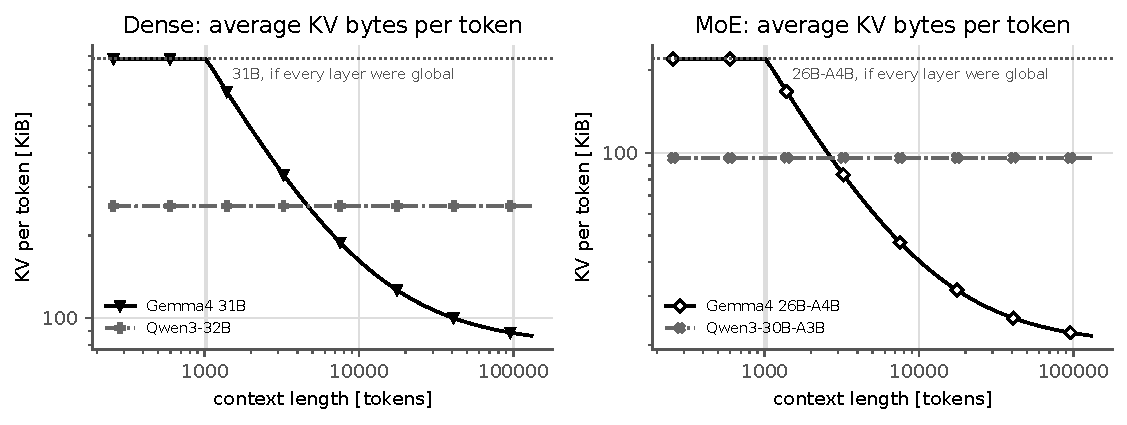
\includegraphics[width=\linewidth]{kv_footprint.pdf}
\caption{1 トークンあたりの平均 KV 量．同クラスの Gemma~4 と Qwen3 の比較で，点線は Gemma~4 の全層を global とした場合．以降のグラフはすべて，マーカーの形でモデルを，塗りつぶしで dense（塗り）/MoE（白抜き）を，線種で Gemma~4（実線）/Qwen3（一点鎖線）を区別する．
window size（1024）を超えると local 層の KV が頭打ちになり，32k では全層 global の場合の約 1/8 に下がる．
一方，window size以下の短いコンテキストでは local 層の KV が大きく，31B は約 4.7k トークン未満で Qwen3-32B より，26B-A4B は約 2.7k トークン未満で Qwen3-30B-A3B より KV が大きい．}
\label{fig:kv}
\end{figure}

%=====================================================================
\section{実験方法}
\label{sec:method}
表\ref{tab:exp} の 9 つの実験を行った．
実験番号は付属リポジトリの \texttt{README.md} と対応しており，実行コマンドとオプションの詳細はそちらとソースコードを参照されたい．

\begin{table}[htbp]\centering\small
\caption{実験の一覧．}
\label{tab:exp}
\begin{tabular}{llL{0.42\linewidth}l}\toprule
番号 & 実験 & 目的 & 結果 \\\midrule
E1 & 単一ストリーム & 同時実行 1 での TTFT・TPOT をプロンプト長ごとに測り，理論下限と比べる & 図\ref{fig:prefill-rate}--\ref{fig:decode-long}，表\ref{tab:measured} \\
E2 & 同時実行数スイープ & 負荷を上げたときのスループットと遅延，帯域の償却を見る & 図\ref{fig:conc-scaling}--\ref{fig:conc-kv} \\
E3 & speculative decoding & MTP の $\gamma$ と生成内容による AL・高速化の変化，n-gram との比較 & 図\ref{fig:mtp}--\ref{fig:mtp-load}，表\ref{tab:spec} \\
E4 & KV 容量 & vLLM が確保する KV 領域と同時実行数の上限を理論値と比べる & 表\ref{tab:kvcap} \\
E5 & マイクロベンチ & 本機で実際に出る GEMM 性能と HBM 帯域を測る & 表\ref{tab:hw} \\
E6 & Nsight Systems & decode 1 ステップの時間をカーネル種別に分解する & 図\ref{fig:nsys-short}，\ref{fig:nsys-long}，\ref{fig:nsys-mtp}，表\ref{tab:nsys} \\
E7 & Nsight Compute & 長コンテキストのAttentionカーネルの律速要因を特定する & 表\ref{tab:ncu} \\
E8 & 追加計測 & Attention backend（Triton）と FP8 KV キャッシュで E1/E2 を測り直し，原因を確かめる．26B-A4B の MTP と E5 の再現性を確かめる & 表\ref{tab:hw}，\ref{tab:backend}，\S\ref{sec:conc} \\
E9 & カーネル解析と修正 & decode の Attention・GEMM カーネルを単体で測り，split-KV を修正した FA4 で E1・E2（31B）・E6 を測り直す & 図\ref{fig:gemv}，\ref{fig:attn-kernel}，表\ref{tab:ctx}，\ref{tab:attn-bw}，\S\ref{sec:ctx-fix} \\
\bottomrule\end{tabular}
\end{table}

\paragraph{サーバと計測（E1--E4）．}
各構成で \texttt{vllm serve} を起動し（BF16，CUDA Graph 有効，最大同時系列数 128，最大長 40{,}960．31B のみ重みが 58\,GiB と大きいため 34{,}816），
クライアントから OpenAI 互換 API にストリーミングでリクエストを送った．
同じプロンプトを繰り返し送るので，TTFT がキャッシュで短くならないよう prefix caching は無効にした．
TTFT は最初のトークンが届くまでの時間，TPOT は（最後のトークンの時刻 $-$ 最初のトークンの時刻）/（出力トークン数 $-1$）である．
speculative decodingの AL は，\texttt{/metrics} のdraft数とaccepted token 数をリクエストの前後で差分して求めた．
なお，オフライン API（\texttt{LLM.generate}）の内部タイムスタンプから求めた TTFT は物理的な下限を下回ったため使っていない．

\paragraph{ワークロード．}
実データとして Babilong と SWE-bench Lite を使い，条件を制御するために合成プロンプトも加えた（表\ref{tab:workload}）．
greedy 生成なので，speculative decodingの有無で出力は同一であり，同じ出力の生成速度を比較できる．

\begin{table}[htbp]\centering\small
\caption{ワークロード．}
\label{tab:workload}
\begin{tabular}{lL{0.42\linewidth}L{0.30\linewidth}}\toprule
名前 & 内容 & ねらい \\\midrule
Synthetic & プロンプト約 256--16k トークン，出力 128 トークン固定，各 3 回 & 長さを細かく制御した掃引 \\
Babilong\cite{babilong} & 長さ 1k--32k $\times$ タスク qa1--qa3 $\times$ 2 件，出力 128 トークン固定 & 実データでの長コンテキスト \\
SWE-bench Lite\cite{swebench} & 8 リポジトリ $\times$ 3 件，パッチ生成（最大 512 トークン） & 自然な生成，ジャンル別のacceptance rate \\
\bottomrule\end{tabular}
\end{table}

同時実行数スイープ（E2）では SWE-bench のプロンプト（平均約 1.3k トークン）を巡回させ，出力 256 トークン固定で同時実行数 $1, 2, \dots, 64$ を測った．

\paragraph{プロファイリング（E5--E7）．}
Nsight Systems では CUDA Graph 内のカーネルもノード単位で記録し，カーネル名から GEMM・MoE・Attention・normalizationなどに分類した．
Nsight Compute では，E2B の約 30k トークン後の decode 1 ステップぶん（Attentionカーネル 35 回）のカウンタを取得した．

%=====================================================================
%=====================================================================
\section{結果}
\label{sec:results}
表\ref{tab:measured} に単一ストリームの代表値と，同時実行スイープでの最大スループットをまとめる．

\begin{table}[htbp]\centering\small
\caption{実測サマリ．TTFT は約 1k と 32k トークンのプロンプト（ms）．prefill MFU（Model FLOPs Utilization）は 8k トークン超のプロンプトでの（モデル FLOPs / TTFT）/ 835\,TFLOPS．
TPOT は 2k トークン未満のプロンプトの中央値（ms），TPOT$_{min}$ は同条件の理論下限，HBM util. は（理論読み出しバイト / TPOT）/ 3.9\,TB/s．
MTP 列は $\gamma=4$ の TPOT 高速化（中央値）とmean acceptance length AL（Synthetic + SWE-bench）．max out tok/s は同時実行スイープでの最大出力スループット．}
\label{tab:measured}
\begin{adjustbox}{max width=\linewidth}
\begin{tabular}{lrrrrrrrrr}
\toprule
Model & TTFT 1k & TTFT 32k & prefill MFU & TPOT & TPOT$_{min}$ & HBM util. & MTP speedup & AL & max out tok/s \\
\midrule
Gemma4 E2B & 22 & 602 & 36\% & 4.21 & 1.19 & 28\% & 1.94$\times$ & 2.78 & 6869 \\
Gemma4 E4B & 25 & 896 & 43\% & 6.23 & 2.42 & 39\% & 2.17$\times$ & 2.90 & 4264 \\
Gemma4 12B & 42 & 2203 & 47\% & 10.41 & 6.19 & 59\% & 1.85$\times$ & 3.20 & 1659 \\
Gemma4 26B-A4B & 35 & 1051 & 33\% & 5.30 & 2.00 & 38\% & 1.35$\times$ & 3.46 & 2392 \\
Gemma4 31B & 104 & 5999 & 45\% & 22.87 & 15.91 & 70\% & 3.08$\times$ & 3.58 & 533 \\
Qwen3-30B-A3B & 45 & 1563 & 41\% & 4.56 & 1.58 & 35\% & -- & -- & 2599 \\
Qwen3-32B & 106 & 7179 & 49\% & 22.01 & 16.45 & 75\% & -- & -- & 839 \\
\bottomrule
\end{tabular}

\end{adjustbox}
\end{table}

%---------------------------------------------------------------------
\subsection{Prefill：Hybrid Attentionは長いプロンプトで効く}
\label{sec:prefill}
\paragraph{大きい dense モデルは本機の GEMM 性能をほぼ使い切っている．}
2k トークン以上の実効 FLOP レートは 12B/31B/Qwen3-32B で 380--415\,TFLOPS にそろう（図\ref{fig:prefill-rate}）．
データシート値の 45--49\% だが，本機の実測 GEMM ピーク（492--514\,TFLOPS，表\ref{tab:hw}）に対しては 74--84\% に当たる．
一方 MoE は 8k トークン超でも 26B-A4B が 265--277\,TFLOPS，Qwen3-30B-A3B が 305--356\,TFLOPS にとどまる．
expert ごとの GEMM（中間次元 704 など）は小さく，プロンプトのトークンが 128 個の expert に分散するため，1 つの GEMM あたりの行数も少なくなるからである．

\begin{figure}[htbp]\centering
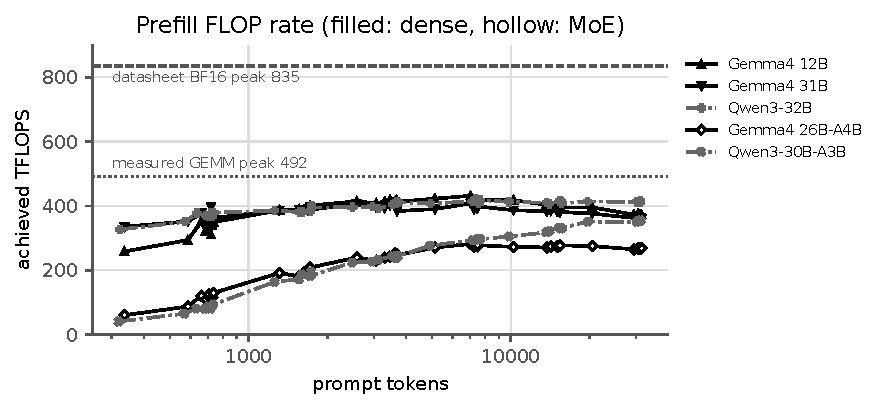
\includegraphics[width=0.6\linewidth]{prefill_rate.pdf}
\caption{prefill の実効 FLOP レート（モデル FLOPs / TTFT）．塗りは dense，白抜きは MoE．破線はデータシート値，点線は本機の実測 GEMM ピーク（初回の計測値 492\,TFLOPS）．}
\label{fig:prefill-rate}
\end{figure}

\paragraph{Hybrid Attentionは長いプロンプトで効く．}
sliding window の効果を確かめるため，同クラスの Qwen3 に対する TTFT の比を，式\eqref{eq:prefill}の FLOPs の比と並べた（図\ref{fig:prefill-hybrid}）．
点線は Gemma~4 の全層を global とした場合の FLOPs の比で，実線との差が sliding window で減った分である．
\begin{itemize}
\item \textbf{window size（1024）以下では差がない．}このとき local 層も全トークンを参照するので，Attentionの FLOPs は Gemma~4 と全層 global で同じになる．
      dense の組では TTFT の比は 0.95--0.98 で，パラメータ数の差による FLOPs の比（0.94）とほぼ一致する．
\item \textbf{効果が見えるのは 4k トークン以上である．}window sizeを超えても，Attentionが prefill の FLOPs に占める割合は 2k トークンで 3\% 程度と小さく，
      sliding window で削れる量も小さい．$P^2$ で増えるAttentionの割合が大きくなる 4k 以上で，実線と点線が離れ，測った TTFT の比も下がっていく．
\item \textbf{32k では 31B が 16\%，26B-A4B が 33\% 速い．}TTFT は 31B が 6.0\,s 対 7.2\,s，26B-A4B が 1.05\,s 対 1.56\,s である．
      Attentionが FLOPs に占める割合は，Qwen3-32B の 36\% に対し 31B は 18\% である．
\end{itemize}
ただし 32k での実測の比（0.84，0.68）は FLOPs の比（0.73，0.51）ほど下がらない．
31B の実効 FLOP レートは 32k で Qwen3-32B より 1 割ほど低く（図\ref{fig:prefill-rate}），Gemma~4 のAttention計算（head dim 512 を含む FA4 系カーネル）の効率が Qwen3 の FlashAttention 3 より低い可能性がある．
また 26B-A4B はwindow size以下の短いプロンプトで FLOPs が多いのに Qwen3-30B-A3B より 15--20\% 速い．この領域の TTFT は 35--50\,ms で計算量では決まっておらず，Attentionとは別の要因である．

\begin{figure}[htbp]\centering
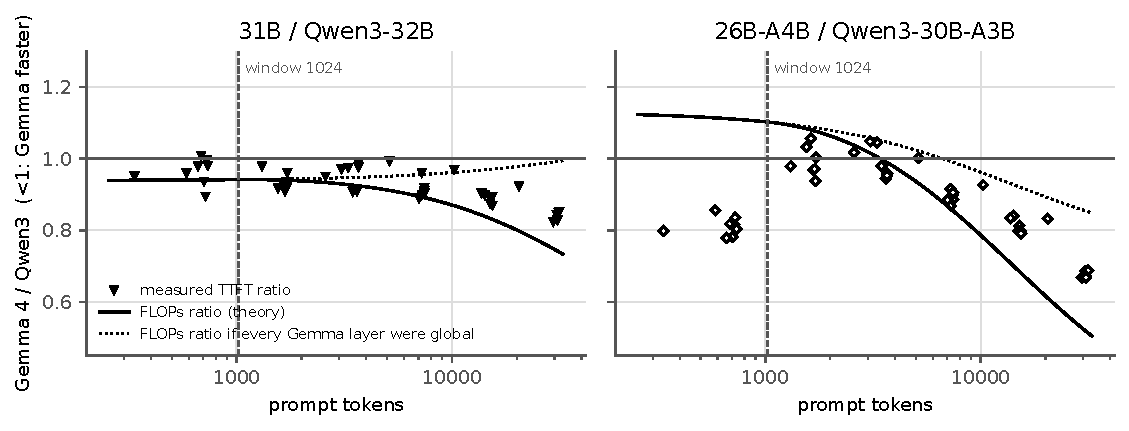
\includegraphics[width=\linewidth]{prefill_hybrid.pdf}
\caption{同クラスの Qwen3 に対する TTFT の比（点）と prefill FLOPs の比（実線）．点線は Gemma~4 の全層を global とした場合の FLOPs の比．破線はwindow size 1024．}
\label{fig:prefill-hybrid}
\end{figure}

%---------------------------------------------------------------------
\subsection{短いコンテキストの decode：大きいモデルほど理論値に近い}
\label{sec:short}
図\ref{fig:decode-bw} のとおり，1 ステップで読むバイト数が大きいモデルほど理論帯域に近い．

\begin{figure}[htbp]\centering
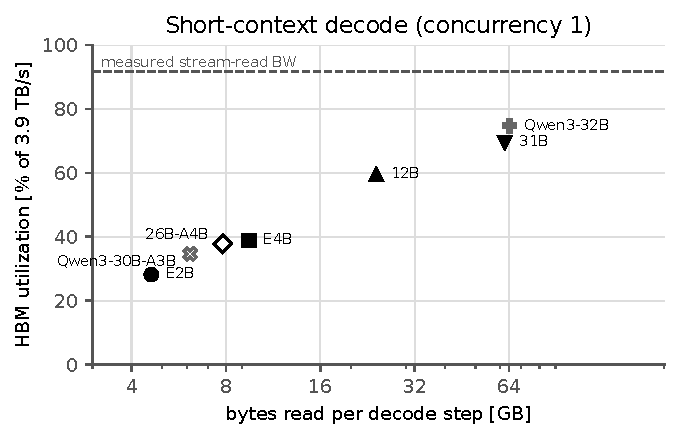
\includegraphics[width=0.6\linewidth]{decode_bw.pdf}
\caption{短いコンテキスト（2k トークン未満）の decode における，1 ステップの読み出しバイト（式\eqref{eq:bytes}）と HBM 利用率．}
\label{fig:decode-bw}
\end{figure}

理由を調べるため，Nsight Systems で測った decode 1 ステップの時間を，
「重みを実測帯域（3.57\,TB/s）で読む理想時間」と，それを超える部分に分けた（図\ref{fig:decode-gap}，表\ref{tab:nsys}）．
\textbf{理想時間を超える部分は，モデルの大きさによらず 1 ステップ 2.7--4.6\,ms ある．}
31B ではこれが理想時間 17.2\,ms の 27\% にすぎないが，E2B では理想時間 1.3\,ms の 2 倍になる．
小さいモデルの帯域利用率が低いのは，この一定の上乗せが相対的に重いためである．

\begin{figure}[htbp]\centering
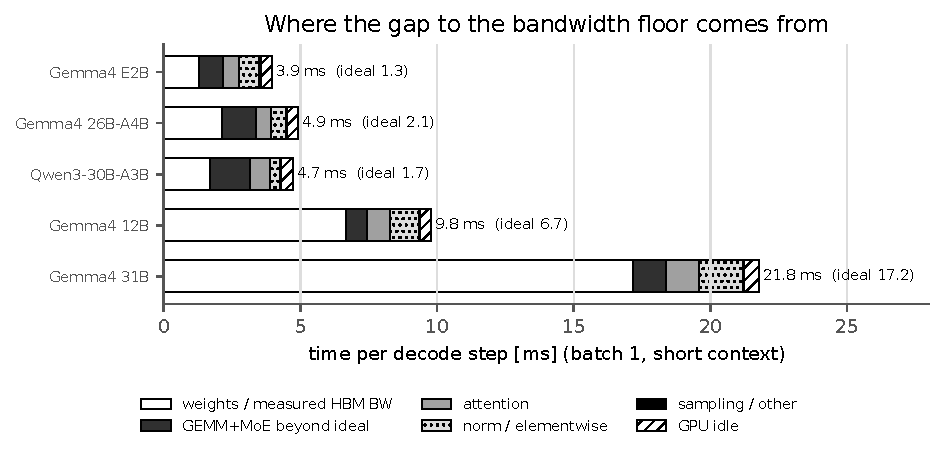
\includegraphics[width=0.85\linewidth]{decode_gap.pdf}
\caption{decode 1 ステップの時間の分解（Nsight Systems，バッチ 1，短いコンテキスト）．白は重みを実測 HBM 帯域で読む理想時間で，それ以外が帯域律速の下限からの差．}
\label{fig:decode-gap}
\end{figure}

上乗せの中身は次のとおりで，いずれも「1 個あたり数 µs かかるカーネルが 1 ステップに数百個並ぶ」ことに由来する．
CUDA Graph により CPU からのカーネル起動のコストはほぼ消えているが，GPU 上でカーネル 1 個ごとにかかる起動・終了の時間とカーネル間の隙間は残る．



\begin{table}[htbp]\centering\small
\caption{decode 1 ステップの時間内訳（ms，バッチ 1，短いコンテキスト）．実効帯域 = 理論重みバイト / GEMM+MoE 時間．}
\label{tab:nsys}
\begin{tabular}{lrrrrrr}\toprule
 & step & GEMM+MoE & 実効帯域 & attention & norm/elem. & idle \\\midrule
Gemma4 E2B & 3.98 & 2.15 & 2.14\,TB/s & 0.61 & 0.74 & 0.40 \\
Gemma4 12B & 9.79 & 7.43 & 3.21\,TB/s & 0.86 & 1.03 & 0.41 \\
Gemma4 26B-A4B & 4.91 & 3.38 & 2.26\,TB/s & 0.52 & 0.56 & 0.40 \\
Gemma4 31B & 21.78 & 18.39 & 3.34\,TB/s & 1.19 & 1.60 & 0.55 \\
Qwen3-30B-A3B & 4.72 & 3.17 & 1.92\,TB/s & 0.73 & 0.34 & 0.44 \\\bottomrule
\end{tabular}
\end{table}

\begin{figure}[htbp]\centering
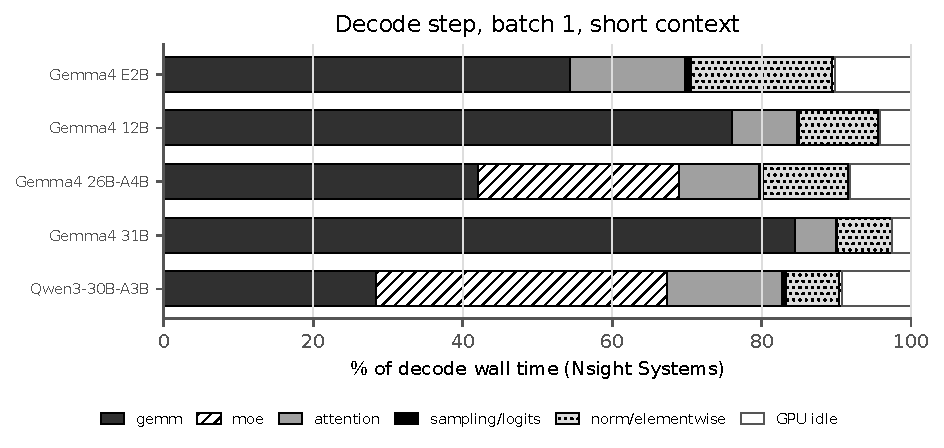
\includegraphics[width=0.85\linewidth]{nsys_short.pdf}
\caption{decode 1 ステップの時間内訳（Nsight Systems，バッチ 1，短いコンテキスト）．白は GPU idle．}
\label{fig:nsys-short}
\end{figure}

\begin{itemize}
\item \textbf{31B の GEMM は帯域をほぼ使い切っている．}重み 61\,GB を 18.4\,ms で読み，3.34\,TB/s（実測ピークの 94\%）に達する．
      TPOT 全体では理論帯域の 70\% で，残りはnormalizationなど（1.6\,ms），Attention（1.2\,ms），idle（0.55\,ms）である．
\item \textbf{E2B は GEMM 自体も帯域を使い切れない．}1 トークンあたり約 585 個のカーネルが走る．
      Nsight Systems によると，最も時間を使う GEMM カーネルは 1 回 6\,µs，grid は平均 43 CTA である．
      \S\ref{sec:gpu-model} で見たとおり，132 SM のうち 89 個に仕事がなく，1 wave で終わってしまう（図\ref{fig:smfill}(a)）．
      hidden 1536 の行列は小さく，CTA に分けても SM の数に届かないためで，GEMM は理想時間より 0.86\,ms 長い．
      さらに RMSNorm やresidual addなどの小さなカーネルが 0.74\,ms，35 層分のAttentionが 0.60\,ms，GPU idleが 0.40\,ms かかる．
\item \textbf{MoE の expert 計算は帯域効率が低い．}26B-A4B と Qwen3-30B-A3B では GEMM+MoE が理想時間より 1.2--1.5\,ms 長く，実効帯域は 1.9--2.3\,TB/s にとどまる．expert 1 つあたりの行列（$704 \times 2816$ など）が小さいためである．
\end{itemize}

\paragraph{GEMM 1 個ごとの固定時間（E9）．}
この上乗せをハードウェアの側から確かめるため，decode と同じ $M=1$ の GEMM を CUDA Graph の中で重みの大きさを変えて測った（図\ref{fig:gemv}）．
重みは L2（60\,MiB）より大きな組を巡回させ，毎回 HBM から読ませている．
時間は $t \approx 3.8\,\mu\text{s} + W / 3.46\,\text{TB/s}$（$W$ は重みのバイト数，$K=1536$ で最小二乗）でよく近似できる．
空のカーネルは 1.1\,µs なので，残りの約 2.7\,µs は最初のデータが HBM から届くまでの latency と，CTA が少なく帯域が立ち上がりきらない時間である．
このため 6\,MB の行列では 1.1\,TB/s しか出ず，HBM 帯域に近づくには 1 回で 50\,MB 以上を読む必要がある．
1 ステップの GEMM の数は E2B が 212 個，12B が 193 個，31B が 241 個で，モデルの大きさによらずほぼ同じである．
この式で 1 ステップの GEMM 時間を予測すると，E2B が 2.13\,ms（実測 2.15\,ms），12B が 7.6\,ms（7.4\,ms），31B が 18.7\,ms（18.4\,ms）で，3\% 以内で一致する．
固定分は E2B では 0.80\,ms で重みの読み出し（1.33\,ms）の 6 割に当たるが，31B では 0.91\,ms で 17.7\,ms の 5\% にすぎない．
\textbf{小さいモデルの帯域利用率が低いのは，約 200 個の GEMM がそれぞれ約 4\,µs の固定時間を払い，読むバイト数が少ないほどその比率が大きくなるからである．}

\begin{figure}[htbp]\centering
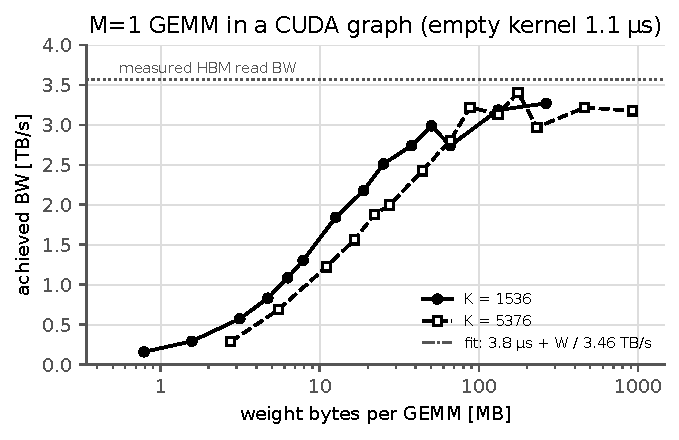
\includegraphics[width=0.6\linewidth]{gemv_bw.pdf}
\caption{$M=1$ の GEMM（CUDA Graph 内，重みは毎回 HBM から読む）の重みの大きさと達成帯域．一点鎖線は $K=1536$ での $t = t_0 + W/\text{BW}$ の当てはめ．}
\label{fig:gemv}
\end{figure}

%---------------------------------------------------------------------
\subsection{長いコンテキストの decode：Attentionカーネルの split-KV のバグ}
\label{sec:ctx}
コンテキスト長に対する TPOT の増え方は，Gemma と Qwen で大きく異なる（図\ref{fig:decode-long}，表\ref{tab:ctx}）．
Qwen3 の増分は KV 読み出しの理論増分の 1.3--1.4 倍に収まるが，Gemma~4 は 26--120 倍である．
理論下限（点線）はどちらもほぼ平らなので，この増分は KV の読み出し量では説明できない．
以下で示すとおり，原因は vLLM 0.32.0 の FlashAttention-4 カーネルの split-KV のバグで，1 行の修正で増分はほぼ理論値まで下がる（表\ref{tab:ctx} の右 2 列）．

\begin{figure}[htbp]\centering
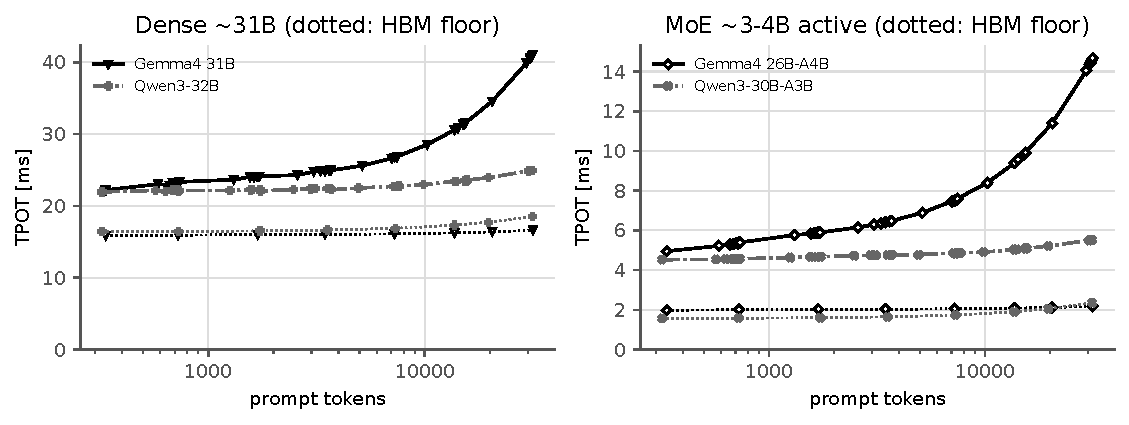
\includegraphics[width=\linewidth]{decode_long.pdf}
\caption{TPOT とプロンプト長．同クラスの Gemma~4 と Qwen3 の比較（点線は式\eqref{eq:bytes}による帯域律速の下限）．}
\label{fig:decode-long}
\end{figure}

\begin{table}[htbp]\centering\small
\caption{TPOT のコンテキスト長依存性（ms）．理論増分は KV 読み出しの増分 / 3.9\,TB/s．
右 2 列は split-KV を修正した FA4（\S\ref{sec:ctx-fix}）で同じ条件を測り直した値（E9）．}
\label{tab:ctx}
\begin{tabular}{lrrrrrr}\toprule
 & \multicolumn{3}{c}{vLLM 0.32.0} & & \multicolumn{2}{c}{split-KV 修正後} \\\cmidrule(lr){2-4}\cmidrule(lr){6-7}
モデル & TPOT（<1k） & TPOT（$\sim$30k） & 増分 & 理論増分 & TPOT（$\sim$30k） & 増分 \\\midrule
Gemma4 E2B & 4.21 & 16.96 & +12.8 & +0.11 & 3.70 & +0.11 \\
Gemma4 E4B & 6.23 & 19.02 & +12.8 & +0.22 & 5.79 & +0.26 \\
Gemma4 12B & 10.41 & 23.96 & +13.6 & +0.15 & 9.93 & +0.21 \\
Gemma4 26B-A4B & 5.30 & 14.44 & +9.1 & +0.17 & 4.87 & +0.14 \\
Gemma4 31B & 22.96 & 40.66 & +17.7 & +0.69 & 23.27 & +1.25 \\
Qwen3-30B-A3B & 4.56 & 5.52 & +1.0 & +0.77 & -- & -- \\
Qwen3-32B & 22.01 & 24.93 & +2.9 & +2.05 & -- & -- \\\bottomrule
\end{tabular}
\end{table}

\paragraph{どのカーネルが遅いか（Nsight Systems）．}
E2B の 30k トークン後の decode では，1 ステップ 19.0\,ms の 79\% をAttentionカーネルが占める（図\ref{fig:nsys-long}）．
同じ FlashAttention-4 カーネルが local 層では 1 回 23\,µs，global 層では 1 回 1.84\,ms かかる．
global 層 1 回で読む KV は約 61\,MB なので，実効帯域は約 33\,GB/s（HBM の 1\%）にすぎない．
31B（約 26k トークン）でも global 層は 1 回 1.56\,ms で，KV ヘッドが E2B の 4 倍あるのに時間はほぼ同じである．
\textbf{時間を決めているのは読むバイト数ではない}ことを示している．
vLLM は head dim が 256 と 512 の層が混在する Gemma~4 に対して全層で FlashAttention-4 を使っており，global 層の decode もこの経路を通る．
理由はコード\ref{lst:fa4}のとおりで，Hopper 既定の FlashAttention 3 は head dim 256 までしか扱えないため，BF16 の KV キャッシュでは FA4 を全層に使う．
FP8 の KV キャッシュを使う場合だけ，head dim 256 の local 層に FA3 を使う層ごとの選択に切り替わる（global 層は FA4 のまま．結果は後述）．

\lstinputlisting[float=htbp, caption={vLLM が Gemma~4 のAttentionカーネルを選ぶ処理（抜粋）．}, label={lst:fa4}]{code/fa4.py}


\begin{figure}[htbp]\centering
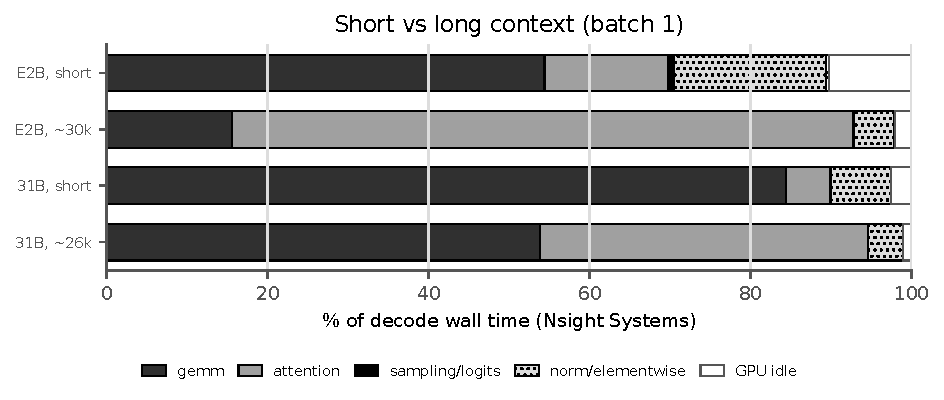
\includegraphics[width=0.85\linewidth]{nsys_long.pdf}
\caption{短いコンテキストと長いコンテキストでの decode 1 ステップの時間内訳（Nsight Systems，バッチ 1）．}
\label{fig:nsys-long}
\end{figure}

表\ref{tab:attn-bw} に，Attentionカーネル 1 回の時間を KV の読み出し量と比べた．
Gemma~4 の global 層は KV を理論帯域で読む時間の 28--117 倍かかり，実効帯域は 33--137\,GB/s にすぎない．
一方 Qwen3-32B（FlashAttention 3，head dim 128）は，26k トークンで 1 層あたり 106\,MB の KV を 44\,µs で読んでおり，実効帯域は 2.4\,TB/s である（split-KV の部分結果をまとめるカーネル 5\,µs を含めても 2.2\,TB/s）．
\textbf{読むバイト数が少ないのに遅いのは，モデルの設計ではなく，Gemma~4 の global 層に使われているAttentionカーネルの実装に原因がある．}

\begin{table}[htbp]\centering\small
\caption{長いコンテキストの decode におけるAttentionカーネル 1 回の時間と KV の読み出し量．理論時間は KV / 3.9\,TB/s．
Gemma~4 は CuTe DSL の FA（FA4 系），Qwen3-32B は FlashAttention 3．修正後の時間は split の部分結果をまとめる combine カーネルを含む（E9）．}
\label{tab:attn-bw}
\begin{tabular}{llrrrrrr}\toprule
 & & & & \multicolumn{2}{c}{vLLM 0.32.0} & \multicolumn{2}{c}{split-KV 修正後} \\\cmidrule(lr){5-6}\cmidrule(lr){7-8}
モデル & 層 & KV / 回 & 理論 & 実測 & 実効帯域 & 実測 & 実効帯域 \\\midrule
Gemma4 E2B（30k） & global & 61\,MB & 16\,µs & 1.84\,ms & 33\,GB/s & 44\,µs & 1.4\,TB/s \\
Gemma4 E2B（30k） & local & 0.5\,MB & 0.1\,µs & 23\,µs & 22\,GB/s & 15\,µs & 33\,GB/s \\
Gemma4 31B（26k） & global & 213\,MB & 55\,µs & 1.56\,ms & 137\,GB/s & 98\,µs & 2.2\,TB/s \\
Gemma4 31B（26k） & local & 17\,MB & 4\,µs & 38\,µs & 440\,GB/s & 23\,µs & 0.74\,TB/s \\
Qwen3-32B（26k） & 全層 & 106\,MB & 27\,µs & 44\,µs & 2.4\,TB/s & -- & -- \\\bottomrule
\end{tabular}
\end{table}

\paragraph{なぜ遅いか（Nsight Compute）．}
global 層のカーネルは理論どおりの 61.6\,MB を読んでおり，余計な読み出しはない（表\ref{tab:ncu}）．
しかし DRAM も SM もピークの 1\% 未満しか使っておらず，メモリ律速でも計算律速でもない．
grid は 128 CTA で SM の数に近いので，一見すると SM は埋まっているように見える．
ところが同じカーネルを単独で Nsight Compute にかけ，SM ごとの稼働サイクル（\texttt{sm\_\_cycles\_active}）を見ると，
最大の SM は 274 万サイクルとカーネルの実行時間（305 万サイクル）のほぼ全体で動いているのに，平均は 3.6 万サイクル，最小は 0 である．
\textbf{128 個の CTA のうち 1 個だけがすべての KV を読み，残りの 127 個は何もせずに終わっている}（図\ref{fig:smfill}(b)）．
実際，1.84\,ms という時間は，修正後のカーネルを split 数 1（CTA 1 個）で動かしたときの時間（1.87\,ms，図\ref{fig:attn-kernel} 右）とほぼ同じである．
31B の global 層は KV ヘッドが 4 本で，仕事をする CTA も 4 個になるため，実効帯域は約 4 倍の 137\,GB/s になる（表\ref{tab:attn-bw}）．

\paragraph{原因：split-KV の分割数が渡っていない．}
decode ではクエリが 1 トークンしかないので，FlashAttention は KV を系列方向に $N$ 個に分け（split-KV），$N$ 個の CTA が並列に部分結果を計算し，最後に combine カーネルでまとめる．
vLLM 0.32.0 に同梱されている FA4（CuTe DSL）の Hopper 向け forward カーネル（\texttt{flash\_fwd\_sm90.py}）では，
各 CTA が自分の担当範囲を計算する \texttt{BlockInfo} を作るときに分割数 \texttt{num\_splits} を渡していない（既定値 1 になる）．
範囲の計算（\texttt{get\_n\_block\_min\_max}）はこの値を使うので，split 0 には KV 全体が，split 1--127 には空の範囲が割り当てられる．
combine カーネルは空の部分結果を無視するので\textbf{出力は正しく}，そのためにこのバグは表に出にくい．
修正は \texttt{BlockInfo} の生成に \texttt{num\_splits=num\_splits} の 1 行を足すだけである．
カーネル単体で測ると，修正前は split 数を 1 から 128 まで変えても時間が 1.87\,ms で変わらないのに対し，修正後は split 数にほぼ反比例して縮み，128 split で 49\,µs（38 倍速，1.26\,TB/s）になる（図\ref{fig:attn-kernel}）．
head dim 256 の FA3 に対しても，読むバイトあたりで同等以上の速さになる．

\begin{table}[htbp]\centering\small
\caption{Nsight Compute：E2B，約 30k トークン後の decode の FlashAttention-4 カーネル（1 ステップ分 35 回の平均）．
CuTe DSL カーネルのためアプリケーションリプレイ・eager 実行・ベースクロック固定で計測しており，絶対時間は Nsight Systems より長い．}
\label{tab:ncu}
\begin{tabular}{lrr}\toprule
 & local 層（28 回） & global 層（7 回） \\\midrule
グリッド / ブロック & 128 CTA / 384 thr & 128 CTA / 384 thr \\
実行時間（ベースクロック） & 37\,µs & 2.78\,ms \\
DRAM 読み出し & 0.63\,MB & 61.6\,MB（理論 61.4\,MB） \\
DRAM スループット（ピーク比） & 0.43\% & 0.58\% \\
SM スループット（ピーク比） & 9.0\% & 0.47\% \\
アクティブ warp（ピーク比） & 17\% & 18\% \\\bottomrule
\end{tabular}
\end{table}

\begin{figure}[htbp]\centering
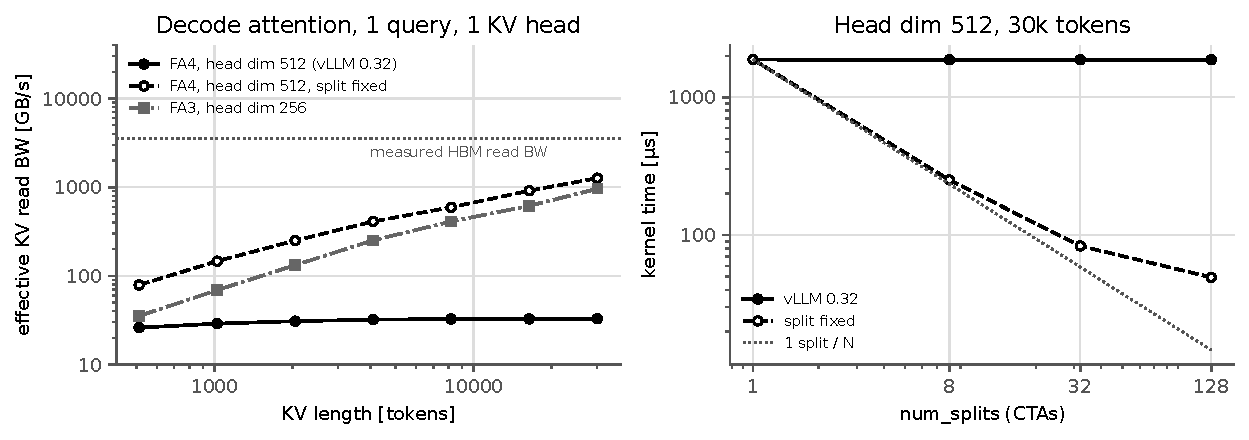
\includegraphics[width=\linewidth]{attn_kernel.pdf}
\caption{global 層（head dim 512）の decode Attention カーネル単体の測定（KV ヘッド 1 本，ページサイズ 16，E9）．
左：KV 長と実効帯域．vLLM 0.32.0 の FA4 は KV 長によらず 1 SM 分の帯域（約 33\,GB/s）で頭打ちになる．
右：30k トークンでの split 数と時間．修正前は split 数を増やしても時間が変わらない．点線は 1 split の時間を split 数で割った理想．}
\label{fig:attn-kernel}
\end{figure}

\paragraph{Attention backend を替えると decode は速くなるが，prefill は遅くなる．}
バグを特定する前に，原因がこのカーネルにあることを確かめるため，同じモデルを Triton の Attention backend（\texttt{-{}-attention-backend TRITON\_ATTN}）で測り直した（E8，表\ref{tab:backend}）．
30k での TPOT は E2B で 17.0\,ms から 6.7\,ms（2.5 倍速），31B で 40.7\,ms から 27.5\,ms（1.5 倍速）に縮んだ．
一方で 32k の TTFT は E2B で 1.9 倍，31B で 1.65 倍に伸びる．prefill では FA4 の方が Triton より速いからである．
FP8 の KV キャッシュでは local 層が FA3 に替わるが，31B の 30k での TPOT は 41.0\,ms で変わらなかった．時間の大半を占める global 層が FA4 のままだからである
（E2B は FP8 KV キャッシュでは CUDA Graph の取り込み中にエラーとなり，起動しなかった）．

\subsection{split-KV を修正した FA4 での測り直し}
\label{sec:ctx-fix}
修正の効果をサービング全体で確かめるため，1 行の修正を入れた FA4 で E1 の単一ストリーム計測と E6 の長いコンテキストのプロファイルを測り直した（E9）．
インストールした vLLM 自体は書き換えておらず，計測用のサーバプロセスの中でだけ，範囲を計算する関数を修正版に差し替えている．
それ以外の条件（モデル，オプション，ワークロード）は元の計測と同じである．

\begin{itemize}
\item \textbf{長いコンテキストの decode の遅さはほぼ消えた．}30k での TPOT は E2B で 17.0\,ms から 3.7\,ms（4.6 倍速），31B で 40.7\,ms から 23.3\,ms（1.7 倍速）になった（表\ref{tab:ctx}，\ref{tab:backend}）．
      TPOT の増分は 0.1--1.3\,ms で，KV 読み出しの理論増分の 0.8--1.8 倍に収まり，Qwen3 と同じ水準になった．
\item \textbf{カーネル 1 回の時間は 16--42 倍短くなった．}global 層 1 回は E2B で 1.84\,ms から 44\,µs，31B で 1.57\,ms から 98\,µs になり（combine を含む），実効帯域は 1.4--2.2\,TB/s に上がった（表\ref{tab:attn-bw}）．
      E2B の 30k での decode 1 ステップに Attention が占める割合は 81\% から 17\% に下がった．
\item \textbf{短いコンテキストの decode も 0.6--1.0\,ms 速くなった．}local 層のカーネルも 128 split のうち 1 個しか働いていなかったからで，E2B の local 層 1 回は 26\,µs から 15\,µs になった．
\item \textbf{prefill と精度は変わらない．}TTFT の差は 32k で $+2$--$6\%$ にとどまり，Babilong の正答数も同じだった（E2B のみ 36 問中 16 問から 15 問）．
      split の部分結果をまとめる順序が変わるため，BF16 の丸めの違いで greedy 生成の出力が途中から分かれるリクエストはある．
\item \textbf{Triton backend より decode も prefill も速い．}修正後の FA4 は 30k の TPOT で Triton を E2B で 1.8 倍，31B で 1.2 倍上回る．
      Triton で decode が速くなったのは Triton が速いからではなく，FA4 が壊れていたからである．
\item \textbf{高並列のスループットは変わらない．}31B の同時実行スイープ（E2）でも，修正後の出力スループットは 32 並列で 507\,tok/s，64 並列で 494\,tok/s で，修正前（533，522\,tok/s）と同程度だった．
      SWE-bench のプロンプトは 1.3k トークン程度と短く，global 層の Attention が時間に占める割合が小さいからで，\S\ref{sec:conc} の頭打ちの原因はこのバグではない．
\end{itemize}

\begin{table}[htbp]\centering\small
\caption{Attention backend と KV キャッシュの型による TPOT と TTFT の違い（ms，中央値）．TPOT（<1k）は 1k トークン未満のプロンプト，$\sim$30k と TTFT は Babilong の各長さ設定（32k 設定は約 31k トークン）．}
\label{tab:backend}
\begin{tabular}{llrrrr}\toprule
モデル & Attention backend & TPOT（<1k） & TPOT（$\sim$30k） & TTFT（8k） & TTFT（32k） \\\midrule
Gemma4 E2B & FA4（既定） & 4.20 & 16.96 & 105 & 602 \\
Gemma4 E2B & Triton & 3.51 & 6.73 & 150 & 1{,}122 \\
Gemma4 E2B & FA4（split-KV 修正後） & 3.59 & 3.70 & 108 & 613 \\
Gemma4 31B & FA4（既定） & 23.01 & 40.66 & 1{,}167 & 5{,}999 \\
Gemma4 31B & Triton & 21.85 & 27.53 & 1{,}529 & 9{,}915 \\
Gemma4 31B & FA3/FA4（FP8 KV） & 23.04 & 40.99 & 1{,}214 & 6{,}185 \\
Gemma4 31B & FA4（split-KV 修正後） & 22.02 & 23.27 & 1{,}225 & 6{,}309 \\
Qwen3-32B & FA3（既定） & 22.00 & 24.93 & 1{,}290 & 7{,}179 \\\bottomrule
\end{tabular}
\end{table}

\textbf{アーキテクチャ上は Gemma~4 の方が長いコンテキストの decode に有利}（30k での KV 読み出しは同クラスの Qwen3 の 28--42\%）であり，
修正後はその利点がそのまま表れる．30k での TPOT は 31B が 23.3\,ms で Qwen3-32B（24.9\,ms）より 7\% 速く，26B-A4B が 4.9\,ms で Qwen3-30B-A3B（5.5\,ms）より 12\% 速い．
vLLM 0.32.0 での「Gemma~4 は長いコンテキストの decode が遅い」という結果は，モデルではなくこのバグによるものだった．

\begin{keybox}{コラム：upstream にコミットするチャンスは，すでに過ぎていた}
このバグを見つけて 1 行の修正で 38 倍速くなったとき，筆者は「これは vLLM にプルリクエストを出せる」と思った．
出力が正しいまま 128 個の CTA のうち 1 個しか働かないという，テストでは見つからない種類のバグであり，Gemma~4 の長いコンテキストの decode を 4.6 倍速くする．
ところが最新の upstream を調べると，すでに直っていた．

\begin{itemize}
\item FA4 のカーネルは vLLM のリポジトリには含まれておらず，ビルド時に vllm-project/flash-attention の特定のコミットを取り込んでいる．
\item そのリポジトリでは 2026 年 9 月 28 日に \textit{Fix SM90 SplitKV block range partitioning}（\#198）として，本書の修正と同じ 1 行の修正がマージされていた．
\item vLLM 側では 10 月 13 日のコミット（\#55866）で取り込むコミットが \texttt{9cd61de} から \texttt{b273a02} に更新され，v0.32.1rc0 以降（v0.33.0rc0/rc1 と main）には修正が入っている．
      このコミットには，head dim 512 の forward の shared memory の競合を直す修正（\#203）も含まれている．
\item 本書で使った v0.32.0 は 10 月 17 日のリリースで，main への修正より後に出ているが，リリース用のブランチには修正が入っておらず，修正前のコミットを取り込んでいる．
      執筆時点で修正を含むのは候補版（rc）だけで，正式リリースの最新版である v0.32.0 を使う利用者はこのバグの影響を受ける．
\end{itemize}

コミットのチャンスだと思ったのにすでに直っていて，正直なところ悔しい．
それでも，このバグがハードウェアの上で何を起こしていたか（1 SM しか働かず，HBM 帯域の 1\% で動いていた）と，修正でサービング性能がどれだけ変わるか（表\ref{tab:ctx}）を定量的に示した報告は，筆者の調べた範囲では見つからなかった．
v0.32.0 で Gemma~4 を長いコンテキストで動かしている場合は，修正を含む版（v0.32.1rc0 以降）に上げれば decode が最大 4.6 倍速くなる．
\end{keybox}

%---------------------------------------------------------------------
\subsection{同時実行：バッチによる償却と，MoE・KV 容量の限界}
\label{sec:conc}
同時実行数スイープ（E2）では，SWE-bench Lite のプロンプト（平均約 1.3k トークン）を出力 256 トークン固定で流した．

\paragraph{バッチで重みの読み出しを償却できる．}
E2B のスループットは同時実行 1 の 189\,tok/s から 64 の 6{,}869\,tok/s（36 倍）まで伸び，TPOT は 4.4\,ms から 7.7\,ms にしか悪化しない（図\ref{fig:conc-scaling} 左）．
重みはバッチ全体で 1 回しか読まないからである．
64 並列でも dense の arithmetic intensity は 30--50\,FLOP/byte で ridge point（138--214）に届かず，decode はまだ帯域律速の領域にある（同右）．
MoE の 2 モデルは 64 並列でも 7--8\,FLOP/byte にとどまる．バッチを大きくすると読む expert も増えるので，FLOPs と読み出しバイトが一緒に増え，比があまり上がらないためである（\S\ref{sec:moe-load}）．

\begin{figure}[htbp]\centering
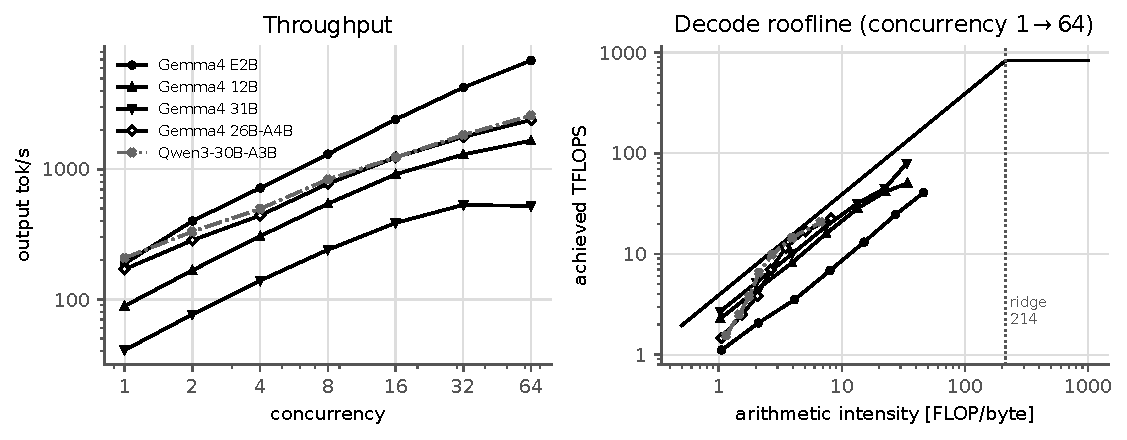
\includegraphics[width=\linewidth]{conc_scaling.pdf}
\caption{同時実行数に対するスループット（左）と，decode ステップのroofline上の位置（右，arithmetic intensityは理論 FLOPs / 理論バイト，到達性能は理論 FLOPs / 実測 TPOT）．dense 3 モデルと MoE 2 モデル．}
\label{fig:conc-scaling}
\end{figure}

\paragraph{高負荷では prefill の計算が TPOT を押し上げる．}
12B の TPOT は 64 並列で 31.6\,ms で，decode だけのroofline下限（11.8\,ms）の 2.7 倍である（図\ref{fig:conc-prefill}）．
chunked prefill では，定常状態で出力 1 トークンあたり約 5 トークン分の新規リクエストの prefill が同じステップに入る．
その計算時間（実測 GEMM ピーク 492\,TFLOPS で 18.0\,ms，514\,TFLOPS なら 17.2\,ms）を，HBM の読み出し時間（11.8\,ms）と重ならずに足し合わせた見積もり（破線，492\,TFLOPS の場合）は 29.0--29.9\,ms になり，
同時実行数による TPOT の増え方をよく再現する．
同時実行 1 でも残る約 4.5\,ms の差は，\S\ref{sec:short} で見た固定的な latencyである．
入力が長く出力が短いワークロードほどこの影響は大きく，prefill/decode の分離や \texttt{max-num-batched-tokens} の調整が効く領域である．

\begin{figure}[htbp]\centering
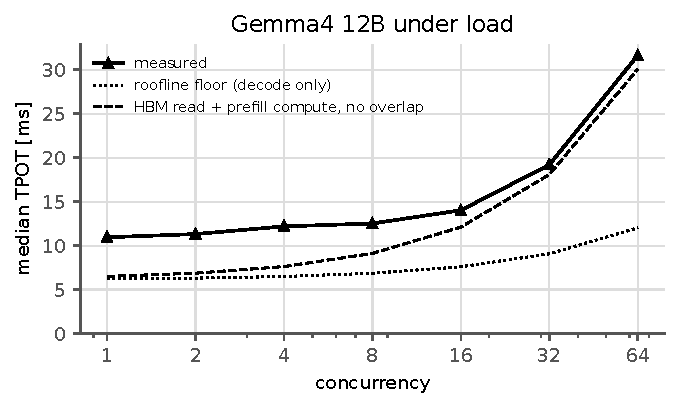
\includegraphics[width=0.6\linewidth]{conc_prefill.pdf}
\caption{12B の TPOT と同時実行数．点線は decode だけのroofline下限，破線は HBM 読み出しと prefill の計算が重ならないとした見積もり．}
\label{fig:conc-prefill}
\end{figure}

\paragraph{MoE の「アクティブ 3.8B」は単一ストリームでのみ成り立つ．}
\label{sec:moe-load}
26B-A4B の TPOT は 5.7\,ms から 23.7\,ms へと急に悪化し，64 並列では dense の 12B に近づく（図\ref{fig:conc-moe}）．
式\eqref{eq:bytes}の $f(B)$ により，1 ステップで読む重みが $B=1$ の 7.7\,GB から $B=64$ で 50\,GB まで増え，12B（24\,GB）の 2 倍になるからである
（expert が等確率・独立に選ばれると仮定した理論値．偏りがあれば実際はこれより少ない）．
Qwen3-30B-A3B も同じ挙動で，最大スループットは 26B-A4B が 2{,}392\,tok/s，Qwen3-30B-A3B が 2{,}599\,tok/s とほぼ同じである．

\begin{figure}[htbp]\centering
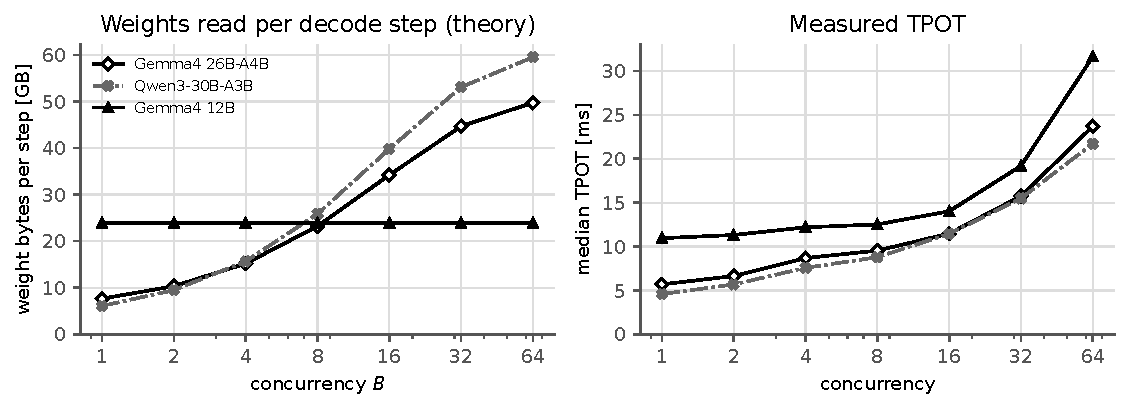
\includegraphics[width=\linewidth]{conc_moe.pdf}
\caption{MoE 2 モデルと dense の 12B について，1 ステップで読む重みの理論値（左，expert が等確率・独立に選ばれると仮定）と実測 TPOT（右）．}
\label{fig:conc-moe}
\end{figure}

\paragraph{31B は 32 並列で頭打ちになり，KV が足りなくなる．}
31B は 32 並列の 533\,tok/s から伸びが止まり，64 並列では TTFT が 18\,s に跳ね上がる（図\ref{fig:conc-kv}）．
サーバログでは KV キャッシュ使用率が 98.6\%，同時に実行されたリクエストは最大 36 本で，残りは待ち行列に入っていた．
重みを載せた後の KV 領域は 27\,GiB しかない．さらに約 1.8k トークンのリクエストはwindow size（1024）を超えて local 層が満杯になるため，1 トークンあたり平均の KV が Qwen3-32B の 2.1 倍（535 対 256\,KiB）になる（図\ref{fig:kv}）．
その結果，64 並列では Qwen3-32B（839\,tok/s）が 31B を 1.6 倍上回った．

\paragraph{FP8 KV キャッシュで容量を倍にしても，スループットは伸びない．}
KV 容量がスループットを決めているのかを確かめるため，31B を FP8 の KV キャッシュで同じ条件で測った（E8）．
KV 領域は 59{,}026 トークンから 114{,}656 トークン（1.94 倍）に増え，64 並列でも 64 本すべてが同時に走るようになった．
その結果 64 並列の TTFT は 18.2\,s から 4.4\,s に縮んだが，TPOT は 52\,ms から 91\,ms に伸び，出力スループットは 522\,tok/s から 527\,tok/s とほとんど変わらなかった．
同時に走るリクエストが最大 36 本から 64 本に増えた分だけ 1 ステップが長くなり，相殺されたのである．
8--32 並列では FP8 KV の方がむしろ 5--9\% 低い（32 並列で 487 対 533\,tok/s）．KV を FP8 に変換する処理や層ごとの backend 切り替えの上乗せと考えられるが，本書では分解していない．
入力を含めた処理トークン数は，64 並列で 31B が約 3{,}000\,tok/s，Qwen3-32B が約 4{,}300\,tok/s である．パラメータ数はほぼ同じなので，31B は 1 トークンを処理する効率そのものが 3 割低い．
したがって \textbf{31B の高並列スループットの頭打ちは KV 容量ではなく，1 ステップの処理の効率で決まっている}．
KV の不足は待ち行列を生んで TTFT を悪化させるが，スループットの上限は決めていない．
\S\ref{sec:ctx} の split-KV のバグを修正してもスループットは変わらなかったので（\S\ref{sec:ctx-fix}），このバグは原因ではない．どのカーネルが効率を下げているかは，本書では分解していない．

\begin{figure}[htbp]\centering
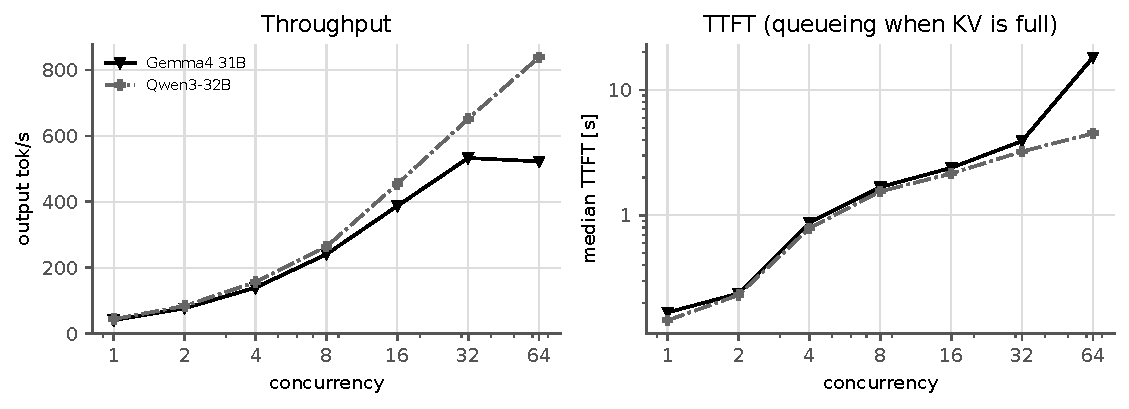
\includegraphics[width=\linewidth]{conc_kv.pdf}
\caption{31B と Qwen3-32B のスループット（左）と TTFT（右）．31B は 32 並列を超えると KV が足りず，リクエストが待ち行列に入る．}
\label{fig:conc-kv}
\end{figure}

\paragraph{vLLM の KV 割り当て（E4）．}
Qwen3 では vLLM が見積もる最大同時実行数が理論値と一致するが，Gemma~4 の 12B/26B/31B では理論値の 1/4--1/6 しか確保されていない（表\ref{tab:kvcap}）．
31B で最大長 32{,}768 の起動に必要と報告された 27.5\,GiB は，全層をフルコンテキストとした場合の理論値（27.50\,GiB）と一致しており，
少なくとも起動時のメモリ見積もりは sliding window の分を差し引いていない．
運用中の割り当てでも，local 層（head dim 256，KV ヘッド 8--16）と global 層（head dim 512，KV ヘッド 1--4）でページの大きさを揃えるためのパディングが理論値との差を生んでいると考えられるが，本書では確認していない．

\begin{table}[htbp]\centering\small
\caption{vLLM が確保する KV 領域と，最大長リクエストの最大同時実行数．ideal は窓と KV 共有を考慮した理論 KV 量（K と V を両方格納）で割った値，no window は全層をフルコンテキストとした場合．}
\label{tab:kvcap}
\begin{adjustbox}{max width=\linewidth}
\begin{tabular}{lrrrrrr}
\toprule
Model & KV pool [GiB] & req. len & ideal KV/req [GiB] & max conc. (vLLM) & max conc. (ideal) & max conc. (no window) \\
\midrule
Gemma4 E2B & 74.2 & 40k & 0.24 & 173.2 & 309 & 105.5 \\
Gemma4 E4B & 68.8 & 40k & 0.64 & 54.2 & 107 & 31.5 \\
Gemma4 12B & 61.0 & 40k & 0.94 & 10.3 & 65 & 4.6 \\
Gemma4 26B-A4B & 35.1 & 40k & 0.98 & 8.6 & 36 & 4.1 \\
Gemma4 31B & 27.0 & 34k & 3.44 & 1.7 & 8 & 0.9 \\
Qwen3-30B-A3B & 27.1 & 40k & 3.75 & 7.2 & 7 & 7.2 \\
Qwen3-32B & 24.8 & 40k & 10.00 & 2.5 & 2 & 2.5 \\
\bottomrule
\end{tabular}

\end{adjustbox}
\end{table}

%---------------------------------------------------------------------
\subsection{MTP Drafter によるspeculative decoding}
\label{sec:mtp}
\begin{table}[htbp]\centering\small
\caption{speculative decodingの方式・draft length別のmean acceptance length AL と TPOT 高速化（中央値）．n-gram はプロンプト内の n-gram 照合（モデル不要）．
Babilong* は出力長を固定するため EOS を抑制しており，回答後に同じ文を繰り返す（acceptance rateが高く出る）ので参考値．}
\label{tab:spec}
\begin{adjustbox}{max width=\linewidth}
\begin{tabular}{llrrrrrr}
\toprule
Model & method & Synthetic AL & Synthetic speedup & SWE-bench AL & SWE-bench speedup & Babilong* AL & Babilong* speedup \\
\midrule
Gemma4 E2B & MTP $\gamma$=1 & 1.63 & 1.46$\times$ & 1.81 & 1.66$\times$ & 1.66 & 1.47$\times$ \\
Gemma4 E2B & MTP $\gamma$=2 & 1.96 & 1.59$\times$ & 2.42 & 2.05$\times$ & 2.07 & 1.62$\times$ \\
Gemma4 E2B & MTP $\gamma$=4 & 2.28 & 1.58$\times$ & 3.22 & 2.37$\times$ & 2.67 & 1.75$\times$ \\
Gemma4 E2B & MTP $\gamma$=8 & 2.46 & 1.33$\times$ & 4.10 & 2.28$\times$ & 3.08 & 1.48$\times$ \\
Gemma4 E4B & MTP $\gamma$=4 & 2.43 & 1.78$\times$ & 3.32 & 2.66$\times$ & 2.19 & 1.60$\times$ \\
Gemma4 12B & MTP $\gamma$=4 & 2.71 & 1.63$\times$ & 3.63 & 1.98$\times$ & 3.41 & 2.15$\times$ \\
Gemma4 26B-A4B & MTP $\gamma$=1 & 1.83 & 1.15$\times$ & 1.85 & 1.03$\times$ & 1.80 & 1.24$\times$ \\
Gemma4 26B-A4B & MTP $\gamma$=2 & 2.45 & 1.28$\times$ & 2.55 & 1.16$\times$ & 2.42 & 1.40$\times$ \\
Gemma4 26B-A4B & MTP $\gamma$=4 & 3.31 & 1.43$\times$ & 3.59 & 1.30$\times$ & 3.24 & 1.37$\times$ \\
Gemma4 26B-A4B & MTP $\gamma$=8 & 4.01 & 1.20$\times$ & 4.58 & 1.15$\times$ & 4.08 & 1.18$\times$ \\
Gemma4 31B & MTP $\gamma$=1 & 1.86 & 1.77$\times$ & 1.86 & 1.79$\times$ & 1.89 & 1.80$\times$ \\
Gemma4 31B & MTP $\gamma$=2 & 2.49 & 2.27$\times$ & 2.57 & 2.37$\times$ & 2.68 & 2.50$\times$ \\
Gemma4 31B & MTP $\gamma$=4 & 3.54 & 3.01$\times$ & 3.61 & 3.14$\times$ & 3.98 & 3.55$\times$ \\
Gemma4 31B & MTP $\gamma$=8 & 4.27 & 3.14$\times$ & 4.55 & 3.59$\times$ & 5.86 & 4.79$\times$ \\
Gemma4 31B & n-gram $\gamma$=4 & 1.03 & 0.95$\times$ & 1.42 & 1.32$\times$ & 3.31 & 3.32$\times$ \\
\bottomrule
\end{tabular}

\end{adjustbox}
\end{table}

\paragraph{AL は似ているのに，高速化は大きく違う．}
$\gamma=4$ の TPOT 高速化は 31B 3.08 倍，E4B 2.17 倍，E2B 1.94 倍，12B 1.85 倍，26B-A4B 1.35 倍である（図\ref{fig:mtp}，Synthetic + SWE-bench）．
31B は vLLM PR の報告（$\gamma=8$ で 3.19 倍）とよく一致する．
一方 AL は 2.8--3.6 トークンとモデル間の差が小さく，26B-A4B は 2 番目に高い．
つまり 26B-A4B が効きにくいのは drafter の予測が外れるからではなく，1 ステップのコスト $c$ が大きいからである（後述）．

\begin{figure}[htbp]\centering
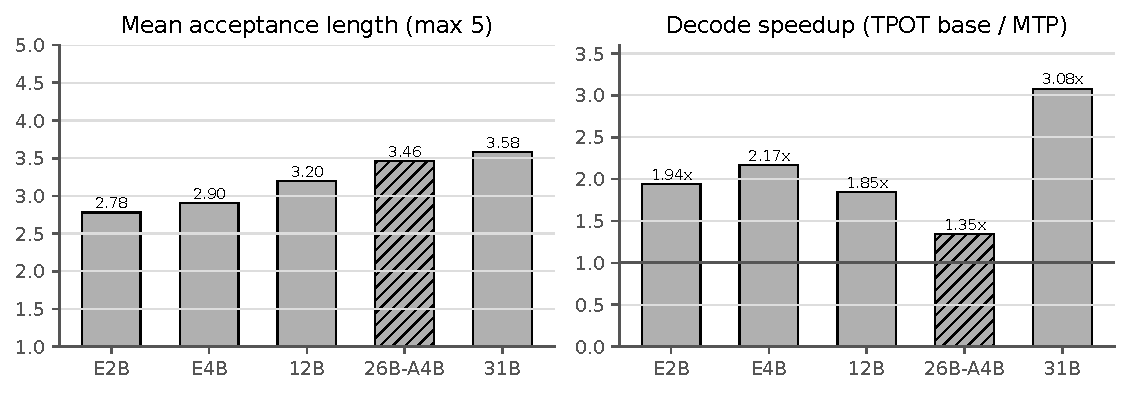
\includegraphics[width=\linewidth]{mtp_speedup.pdf}
\caption{MTP（$\gamma=4$，同時実行 1，Synthetic + SWE-bench）のmean acceptance length（左）と TPOT 高速化（右）．斜線は MoE の 26B-A4B．}
\label{fig:mtp}
\end{figure}

\paragraph{生成内容への依存．}
コードのパッチ生成（SWE-bench）は自然文（Synthetic）より AL が高い（E2B で 3.22 対 2.28）．差分の文脈行はコードのコピーで予測しやすいためである．
リポジトリ別では sympy が最も低く，matplotlib が最も高い（付録の図\ref{fig:genre}）．
モデル不要の n-gram（31B，$\gamma=4$）は，プロンプトからのコピーが多い SWE-bench で 1.32 倍，繰り返しの多い Babilong* で 3.32 倍だが，自由な文章では 0.95 倍とかえって遅くなる（図\ref{fig:mtp-ngram}）．
MTP はどのワークロードでも 3.0--3.5 倍を出しており，\textbf{学習済み drafter の強みは内容によらないacceptance rateにある}．

\begin{figure}[htbp]\centering
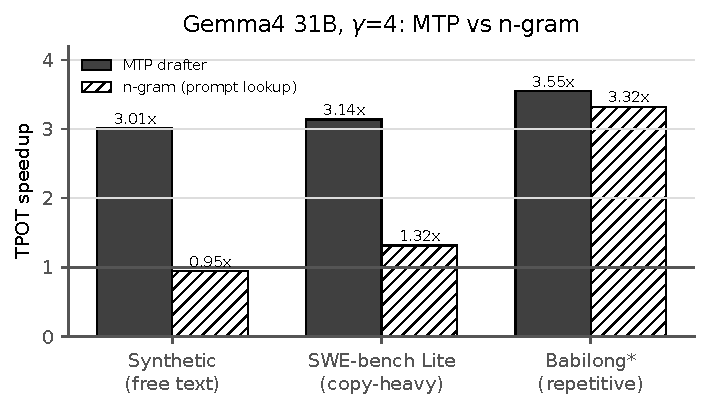
\includegraphics[width=0.62\linewidth]{mtp_vs_ngram.pdf}
\caption{31B（$\gamma=4$）での MTP と n-gram の TPOT 高速化．Babilong* は回答後に同じ文を繰り返すので参考値．}
\label{fig:mtp-ngram}
\end{figure}

\begin{figure}[htbp]\centering
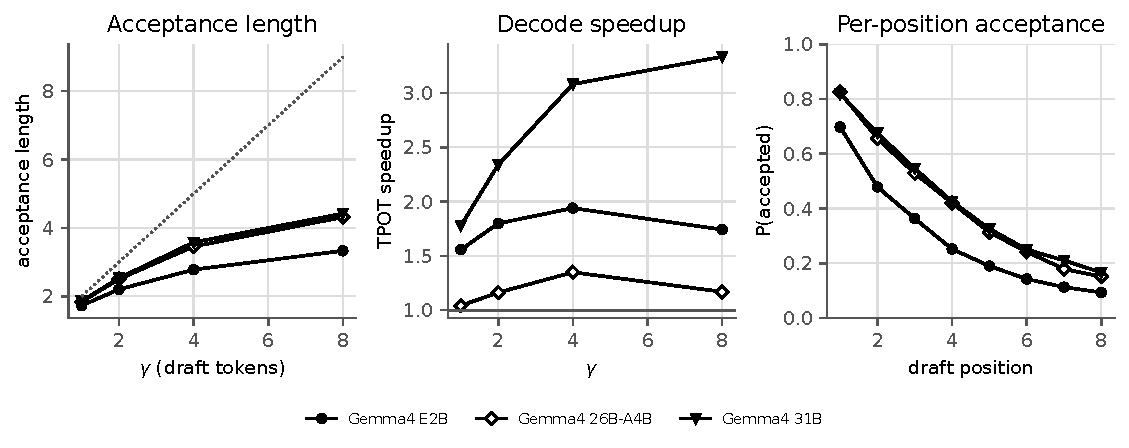
\includegraphics[width=\linewidth]{mtp_gamma.pdf}
\caption{draft length $\gamma$ の影響（Synthetic + SWE-bench）．左：AL（点線は全 acceptの上限 $\gamma+1$），中：TPOT 高速化，右：$\gamma=8$ での位置ごとのacceptance rate．}
\label{fig:gamma}
\end{figure}

\paragraph{なぜ 26B-A4B では効きにくいか：コストモデルによる説明．}
式\eqref{eq:spec}の AL と $c$ を分けると（図\ref{fig:costmodel}），26B-A4B の AL（3.46）は 31B（3.58）とほぼ同じで，差は $c$ にある．
26B-A4B は $\gamma=4$ のverifyで 5 トークン分の expert（一様・独立の仮定で 27.5\%．$B=1$ では 6.3\%）を読むので，verifyだけで通常ステップの 2.3 倍のバイトを読む．
drafter（target の 11\%）4 回分を足すと式\eqref{eq:cpred}で $c_\text{pred}=2.78$ となり，実測の $c=2.56$ と近い．
一方 31B は dense なのでverifyがほぼ無料で，$c_\text{pred}=1.12$（実測 1.16），予測高速化 3.20 倍（実測 3.08 倍）とよく一致する．

E2B/E4B/12B は実測の $c$ が予測より 0.3--0.5 大きい．
E2B/E4B は 1 ステップが 2--4\,ms と短く，drafter 1 回分の固定latencyが相対的に重い．そのため E2B は $\gamma=8$ で $\gamma=4$ より遅くなる．
12B と 26B-A4B では MTP 有効時に GPU が約 50\% の時間idleになっていた（図\ref{fig:nsys-mtp}）．
26B-A4B は別の日に測り直しても，高速化が $\gamma=4$ で 1.41 倍，$\gamma=8$ で 1.24 倍，GPU busy が 48\%（通常の decode は 92\%，31B の MTP は 90\%）で，同じ結果になった（E8）．
drafter の経路で 1 出力トークンあたり CUDA Graph 起動が 12--20 回，通常のカーネル起動が 86--114 回発生しており（通常の decode ではそれぞれ 1.1 回と 25 回），CPU が律速になっている．
drafter の経路を完全に CUDA Graph 化できれば，12B の高速化は 1.85 倍から予測値の 2.7 倍に近づく．
\textbf{最適な $\gamma$ は，大きい dense モデルで 8 以上，小さいモデルで 4 前後，MoE で 4（低負荷時）である．}

\begin{figure}[htbp]\centering
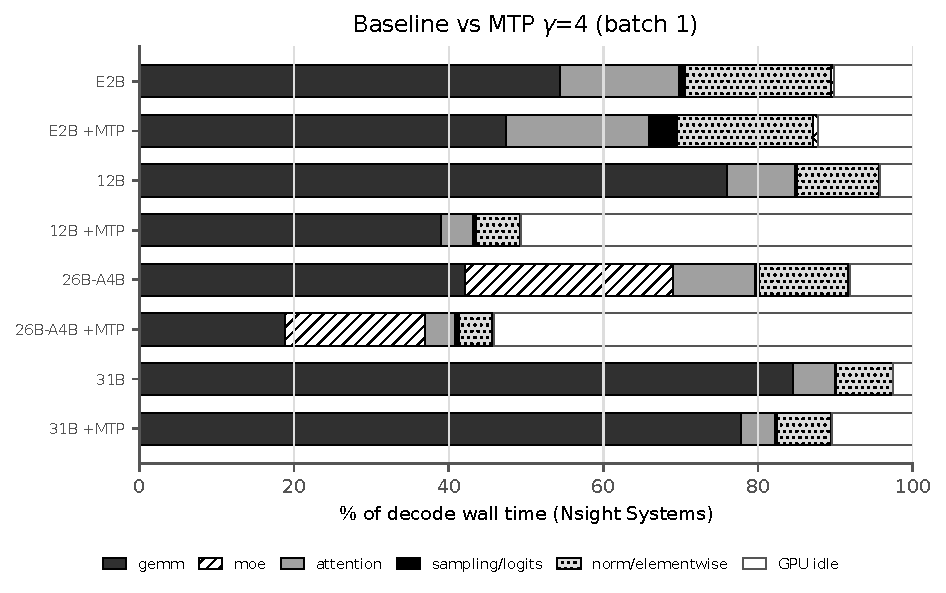
\includegraphics[width=0.85\linewidth]{nsys_mtp.pdf}
\caption{通常の decode と MTP（$\gamma=4$）の時間内訳（Nsight Systems，バッチ 1）．12B と 26B-A4B では MTP 有効時に GPU のidle（白）が約半分を占める．}
\label{fig:nsys-mtp}
\end{figure}

\begin{figure}[htbp]\centering
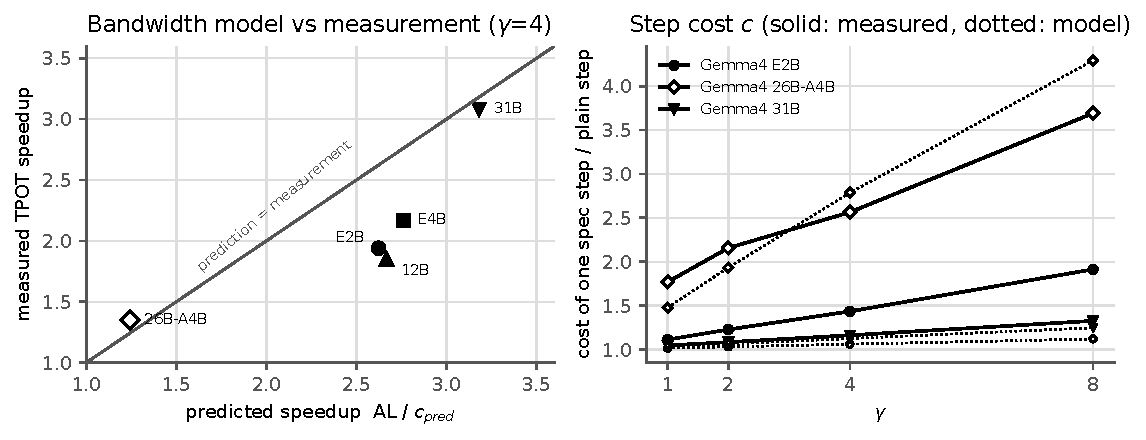
\includegraphics[width=\linewidth]{mtp_cost_model.pdf}
\caption{帯域コストモデルによる予測高速化 AL/$c_\text{pred}$ と実測（左，$\gamma=4$）．$\gamma$ を振った 3 モデルの 1 speculative stepのコスト $c$（右，実線：実測 AL/高速化，点線：式\eqref{eq:cpred}）．}
\label{fig:costmodel}
\end{figure}

\paragraph{高負荷時の MTP．}
同時実行数を上げると dense モデルの MTP の利得は縮む（図\ref{fig:mtp-load}）．E2B では同時実行 1 の 2.3 倍が 64 では 1.16 倍になる．
バッチが大きくなるとarithmetic intensityが上がり，verifyトークン分の計算が無料ではなくなるためである．
逆に 26B-A4B は 1.25 倍から 1.51 倍へと利得が\emph{増える}．高負荷ではもともと expert の大半を読んでいるので，verifyトークンを増やしても読み出しバイトがほとんど増えないからである．
vLLM PR が報告した「26B-A4B では MTP の利得がバッチとともに増える」傾向と一致する．

\begin{figure}[htbp]\centering
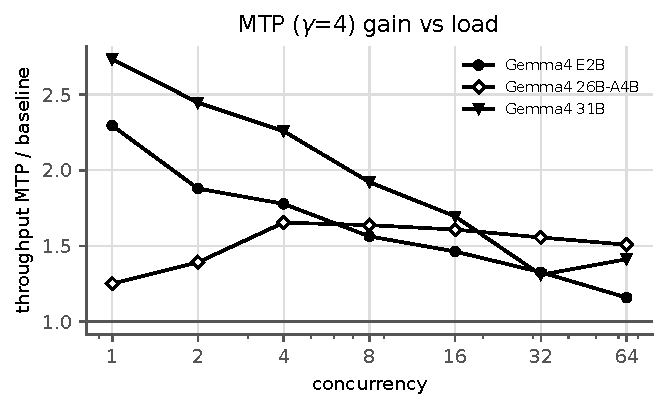
\includegraphics[width=0.6\linewidth]{concurrency_mtp.pdf}
\caption{同時実行数ごとの MTP（$\gamma=4$）のスループット向上率（条件は図\ref{fig:conc-scaling} と同じ）．dense の E2B・31B と MoE の 26B-A4B で傾向が逆になる．}
\label{fig:mtp-load}
\end{figure}

%=====================================================================
\section{外部の結果との比較と総合評価}
\label{sec:discussion}

\subsection{外部の結果と整合しているか}
本書の数値を，vLLM の Gemma~4 MTP 実装 PR\cite{vllmpr}，第三者による H100 でのベンチマーク\cite{jarvislabs,inferencebench}，Google の MTP 紹介記事\cite{mtpblog}と比べた（表\ref{tab:external}）．
外部の測定は GPU（H100 SXM），vLLM のバージョン，Attention backend，ワークロードが本書と異なるので，比べられるのは傾向と桁である．

\begin{table}[htbp]\centering\small
\caption{外部の結果との比較（同時実行 1 は出力 tok/s，括弧内は baseline に対する倍率）．
外部の測定はいずれも H100 SXM（HBM 3.35\,TB/s）と SPEED-Bench を使っており，jarvislabs は Attention backend に Triton を使っている．}
\label{tab:external}
\begin{adjustbox}{max width=\linewidth}
\begin{tabular}{lllll}\toprule
指標 & 本書（H100 NVL，vLLM 0.32） & vLLM PR\cite{vllmpr} & jarvislabs\cite{jarvislabs} & 整合 \\\midrule
31B baseline，同時実行 1 & 42\,tok/s（TPOT 23.6\,ms） & 42.6\,tok/s & 40.3\,tok/s（TPOT 24.4\,ms） & ○ \\
31B MTP $\gamma=8$，同時実行 1 & 148\,tok/s（3.33$\times$） & 136\,tok/s（3.19$\times$） & 125\,tok/s（3.11$\times$） & ○ \\
31B baseline，同時実行 16 & 387\,tok/s（TPOT 32.2\,ms） & -- & 375\,tok/s（TPOT 32.9\,ms） & ○ \\
26B-A4B baseline，同時実行 1 & 175\,tok/s & 169\,tok/s & 177\,tok/s & ○ \\
26B-A4B MTP，同時実行 1 & 226\,tok/s（1.35$\times$，$\gamma=4$） & 270\,tok/s（1.60$\times$，$\gamma=4$） & 264\,tok/s（1.49$\times$，$\gamma=8$） & △ 本書が低い（再計測でも 1.41$\times$） \\
26B-A4B の MTP 利得と負荷 & 1.25$\to$1.51$\times$（同時実行 1$\to$64） & 1.60$\to$2.27$\times$（バッチ 1$\to$64） & -- & ○ 同じ傾向 \\
E4B MTP $\gamma=4$，同時実行 1 & 2.17$\times$ & 1.78$\times$ & -- & △ 本書が高い \\
\bottomrule\end{tabular}
\end{adjustbox}
\end{table}

\begin{itemize}
\item \textbf{31B の baseline と MTP はよく一致する．}baseline の出力速度は 3 つの測定で 40--43\,tok/s，MTP の高速化は 3.1--3.3 倍にそろう．
      同時実行 16 での TPOT も 32--33\,ms で一致する．
      H100 NVL の HBM 帯域は SXM より 16\% 大きいが，31B の baseline はほぼ同じである．重みの読み出しから求めた実効帯域はどちらも約 2.6\,TB/s で，理論帯域に対しては本書が 67\%，SXM が 78\% になる．
      帯域の大きい NVL でも，実際に引き出せる帯域の絶対値は SXM と変わらないことを示唆している．
\item \textbf{26B-A4B の MoE で MTP が効きにくいことも共通している．}Google の記事も 26B の MoE はバッチ 1 で routing が難しく，バッチを増やすと利得が増えると述べており\cite{mtpblog}，vLLM PR の表も同じ傾向を示す．
      これは \S\ref{sec:mtp} のコストモデル（verify で読む expert が増える）と整合する．
      ただし本書の高速化（1.35 倍）は外部（1.49--1.60 倍）より低い．baseline はほぼ同じなので，差は MTP 側にある．
      測り直しても 1.41 倍で外部より低く，baseline の TPOT も $\pm 2\%$ で一致したので，測定のばらつきではない．
      本書では 26B-A4B の MTP 有効時に GPU が約半分 idle になっており（図\ref{fig:nsys-mtp}，再計測でも GPU busy 48\%），CPU 側の処理が律速していた．
      CPU の性能や vLLM のバージョンで CUDA Graph 化される範囲が変わるとこの部分が大きく変わるため，それが差の原因と考えられる．
\item \textbf{高負荷のスループットはワークロードの形で大きく変わる．}inferencebench は H100 SXM の 31B で同時実行 32 のとき 855\,tok/s（入力 2048，出力 1024 トークン）を報告しており\cite{inferencebench}，本書の 533\,tok/s（入力 約 1.3k，出力 256 トークン）より高い．
      出力 1 トークンあたりの prefill 量は先方が 2 トークン，本書が 5.2 トークンであり，\S\ref{sec:results} の prefill 混入の議論から，出力が長いほどスループットが高くなるのは整合する．
\item \textbf{長いコンテキストの decode の遅さを定量的に報告した外部の結果は見つからなかった．}
      原因の split-KV のバグは flash-attention 側で 2026 年 9 月に修正済みで（\S\ref{sec:ctx} のコラム），vLLM v0.32.1rc0 以降には入っている．
      また head dim 512 の global 層が Attention backend の選択を難しくしていることはコミュニティでも知られている．
      vLLM には，head dim 混在のため全層で Triton に切り替わり E4B が RTX 4090 で約 9\,tok/s しか出ないという報告\cite{vllmissue38887}や，local 層だけ FlashAttention を使えるようにする PR\cite{vllmpr38891}（2026 年 10 月時点で未マージ）がある．
      jarvislabs が Triton backend で測っているのに対し，本書の vLLM 0.32 は FA4 を選ぶ（コード\ref{lst:fa4}）など，バージョンによって使われるカーネル自体が変わっている．
      本書でも backend を Triton に替えると 30k での TPOT が 1.5--2.5 倍速くなり，prefill が 1.7--1.9 倍遅くなった（表\ref{tab:backend}）．
\end{itemize}

\subsection{Qwen3 と比べて良い結果か}
結論は，\textbf{アーキテクチャとしては Gemma~4 が優れている点が多いが，現在の vLLM の上ではその一部しか性能に表れておらず，条件によっては Qwen3 に負ける}である．

\begin{table}[htbp]\centering\small
\caption{同クラスの Qwen3 に対する Gemma~4 の評価．○：Gemma~4 が良い，△：同等，×：Gemma~4 が悪い．}
\label{tab:verdict}
\begin{tabular}{L{0.25\linewidth}cL{0.34\linewidth}L{0.24\linewidth}}\toprule
観点 & 評価 & 根拠 & 原因 \\\midrule
長いプロンプトの TTFT & ○ & 32k で 16--33\% 短い & Hybrid Attention（設計） \\
単一ストリームの decode（短いコンテキスト） & △ & 31B 22.9 対 22.0\,ms，26B-A4B 5.3 対 4.6\,ms & ほぼパラメータ数どおり \\
MTP を使った単一ストリームの decode & ○ & 31B は 3.1--3.3 倍で Qwen3-32B（baseline）の約 3 倍速い & 公式 drafter（設計） \\
長いコンテキストの decode & \shortstack{×\\{\scriptsize 修正後 ○}} & v0.32.0 では 30k で TPOT の増分が 9--18\,ms（Qwen3 は 1--3\,ms）．split-KV の修正後は 31B 23.3 対 24.9\,ms，26B-A4B 4.9 対 5.5\,ms & FA4 の split-KV のバグ（実装，v0.32.1rc0 で修正） \\
長いコンテキストの KV 量（理論） & ○ & 32k で 31B 3.3\,GiB 対 8.0\,GiB & Hybrid Attention（設計） \\
短いリクエストの高並列スループット & × & 64 並列で 31B は Qwen3-32B の 0.6 倍．FP8 KV で KV 容量を倍にしても変わらない & 1 トークンの処理効率（実装と考えられる） \\
MoE の高負荷スループット & △ & 2{,}392 対 2{,}599\,tok/s & 両者とも expert の読み出しが増える \\
\bottomrule\end{tabular}
\end{table}

表\ref{tab:verdict}で × がついた 2 点のうち，長いコンテキストの decode は完全に実装の問題であり（1 行の修正で消え，修正後は Qwen3 より速い），
高並列のスループットも KV 容量ではなく 1 トークンの処理効率で決まっていた．
つまり Gemma~4 の「残念な」結果の多くは\textbf{ソフトウェアで直せる}種類のものである．
逆に，○の項目のうち MTP による高速化は vLLM ですでに使え，外部の測定でも再現している．
利用者の立場では，現時点で次のように使い分けるのがよい．
\begin{itemize}
\item \textbf{低負荷・低 latency の対話}：31B + MTP（$\gamma=4$--8）が最も速い．同クラスの Qwen3-32B の約 3 倍の速さで出力できる．
\item \textbf{長いプロンプトを読ませる用途}（RAG，要約，長い文脈での対話）：prefill が速く，split-KV の修正後は decode も Qwen3 より速い Gemma~4 が有利である．
      ただし vLLM v0.32.0 では長いコンテキストの decode が 1.7--4.6 倍遅いので，修正を含む v0.32.1rc0 以降を使う．
      v0.32.0 のまま Attention backend を Triton にする回避策は，decode は速くなるが prefill が 1.7--1.9 倍遅くなり，修正版の FA4 にどちらでも劣る．
\item \textbf{短いリクエストを大量にさばく用途}：31B のスループットは 64 並列で Qwen3-32B の 0.6 倍で，FP8 KV キャッシュでも伸びない．
      FP8 KV キャッシュは待ち行列を消して TTFT を 18\,s から 4.4\,s に縮めるので，TTFT を抑えたい場合には有効である．スループットが重要なら Qwen3-32B が有利である．
\end{itemize}

\subsection{コミュニティとして何をすべきか}
本書の測定から，効果が大きいと見積もれる順に挙げる．
\begin{enumerate}
\item \textbf{split-KV の修正を含む版をリリースし，利用者に知らせる．}
      vLLM v0.32.0 の FA4 は split-KV の分割数が渡っておらず，128 個の CTA のうち 1 個しか働かない（\S\ref{sec:ctx}）．
      修正は flash-attention 側にも vLLM の main にもすでに入っているが，執筆時点の正式リリースは修正前の v0.32.0 である．
      修正すると 30k での TPOT は E2B で 17\,ms から 3.7\,ms，31B で 41\,ms から 23\,ms になる（\S\ref{sec:ctx-fix}）．
      出力が正しいまま遅くなる種類のバグはテストで見つからないので，「split 数を増やすと時間が縮む」ことを確かめる性能テストがあれば再発を防げる．
      Triton backend への切り替えや，local 層だけ FA3 を使う層ごとの選択（PR\cite{vllmpr38891}）は，修正版の FA4 があれば不要になる．
\item \textbf{KV キャッシュ管理の改善．}
      起動時の見積もりが sliding window を差し引いていないこと，運用時の割り当てが理論値の 1/4--1/6 にとどまることを直せば，同じメモリでより多くのリクエストを同時に走らせられる．
      ただし FP8 KV キャッシュで容量を倍にした実験では，待ち行列が消えて TTFT は縮んだがスループットは変わらなかった（\S\ref{sec:conc}）．効果は主に TTFT に表れ，スループットを上げるには 1 ステップの処理効率の改善と組み合わせる必要がある．
      さらに K=V の global 層で RoPE 前の K を 1 本だけ保存すれば，global 層の KV を半分にできる．
\item \textbf{drafter 経路の CUDA Graph 化．}
      12B と 26B-A4B では MTP 有効時に GPU が半分 idle で（26B-A4B は再計測でも GPU busy 48\%），CPU からのカーネル起動が律速している．完全に CUDA Graph 化できれば 12B の MTP は 1.85 倍から帯域モデルの予測（2.7 倍）に近づき，26B-A4B も外部の 1.5--1.6 倍に近づくと考えられる．
      負荷に応じて $\gamma$ を自動で変える仕組みも，dense と MoE で最適値が逆向きに動く（\S\ref{sec:mtp}）ことから有用である．
\item \textbf{ベンチマークの報告のしかた．}
      Gemma~4 は vLLM のバージョンによって Attention backend が Triton，FA4 などと変わり，ワークロードの入出力長でスループットも大きく変わる．
      結果を共有するときは，vLLM のバージョン，Attention backend，入力長・出力長，同時実行数を併記することが，比較できる知見を積み上げるうえで重要である．
\end{enumerate}

%=====================================================================
\clearpage
\section{ボトルネックとチューニングの指針}
\label{sec:tuning}
\begin{table}[H]\centering\small
\caption{ボトルネックと対策のまとめ．}
\label{tab:tuning}
\begin{tabular}{L{0.16\linewidth}L{0.16\linewidth}L{0.29\linewidth}L{0.27\linewidth}}\toprule
対象 & 律速要因 & 根拠 & 有効な対策 \\\midrule
小モデル（E2B/E4B）の decode & カーネルの固定latency & 帯域利用率 28--39\%，1 トークン約 600 カーネル & 同時実行数を上げる（64 並列で 36 倍），MTP（1.9--2.2 倍），normalization・residualのカーネル融合 \\
大 dense（31B）の decode & HBM 帯域 & 帯域利用率 70\%，GEMM は実測ピークの 94\% & 重みの量子化（FP8/INT4），MTP $\gamma \ge 4$（3.1--3.3 倍） \\
MoE（26B-A4B） & 負荷により変化 & 高負荷では読む expert が 25B 相当に増える & 低負荷は MTP の効果が小さい．高負荷では MTP が効く（1.5 倍） \\
長いコンテキストの decode & FA4 の split-KV のバグ（v0.32.0） & 理論値の 26--120 倍，128 CTA のうち 1 個だけが働く & 修正を含む v0.32.1rc0 以降を使う（30k で 1.7--4.6 倍速，TTFT は不変） \\
高並列の TPOT & 混入する prefill の計算 & 12B の 64 並列で 31.6\,ms，HBM 読み出し＋prefill 計算の見積もり 29.9\,ms & prefill/decode の分離，\texttt{max-num-batched-tokens} の調整 \\
KV 容量（高並列） & local 層の KV と vLLM の割り当て & 31B は 1.8k トークンのリクエストで平均 535\,KiB/トークン（Qwen3-32B の 2.1 倍），割り当ては理論値の 1/4--1/6．不足すると待ち行列で TTFT が 18\,s に & FP8 KV キャッシュ（TTFT 18$\to$4.4\,s，スループットは不変），FP8 重み，RoPE 前の K を 1 つだけ格納する K=V の活用 \\
Prefill & 電力制限下の GEMM 性能 & 実測 GEMM ピークの 74--84\% & FP8 GEMM（理論 2 倍） \\
\bottomrule\end{tabular}
\end{table}

%=====================================================================
\section{まとめ}
H100~NVL 1 基・vLLM 0.32 で Gemma~4 ファミリのサービング性能を測り，チェックポイントから求めた理論限界と比べた．
4 つの問いへの答えを，結果とその理由の組でまとめる．

\paragraph{Q1：GPU の性能をどこまで出し切れているか．}
\begin{itemize}
\item 31B の decode は HBM 理論帯域の 70\% に達した．これは GEMM が実測帯域ピークの 94\% で重みを読めており，重みの読み出し以外の上乗せ（1 ステップ約 4.6\,ms）が理想時間 17.2\,ms に対して小さいからである．
\item E2B の decode は 28\% にとどまった．これは重みの読み出し以外に，小さな GEMM・normalizationなどのカーネル群・Attention・GPU idleで 1 ステップ約 2.7\,ms かかり，重みを読む理想時間（1.3\,ms）の 2 倍に達するからである．この上乗せはモデルの大きさによらずほぼ一定なので，読むバイトが少ないモデルほど不利になる．
\item MoE の 26B-A4B は 38\% だった．これは expert 1 つあたりの行列が小さく，expert の GEMM が帯域を使い切れないからである．
\item prefill は実測 GEMM ピークの 74--84\% に達した．データシート値に対して 45--49\% にとどまるのは，H100 NVL が 400\,W の電力制限で大きな GEMM のクロックを下げるからである．同じ理由で GEMM ピーク自体も計測ごとに 492--514\,TFLOPS と揺れた．
\end{itemize}

\paragraph{Q2：アーキテクチャ上の工夫は効いているか．}
\begin{itemize}
\item 32k トークンの TTFT は Qwen3 より 16--33\% 短かった．これはHybrid Attentionによって $P^2$ で増えるAttention計算が global 層だけに限られ，Attentionが FLOPs に占める割合が 36\% から 18\% に下がるからである．window size以下では差がなく，効果はAttentionの割合が大きくなる 4k トークン以上で現れる．
\item 一方，vLLM 0.32.0 では，コンテキストを 30k トークンまで伸ばしたときの TPOT の増分が 9--18\,ms で，Qwen3 の 1--3\,ms を大きく上回った（31B は 41\,ms 対 Qwen3-32B の 25\,ms）．これは FA4 カーネルの split-KV に分割数が渡っておらず，128 個の CTA のうち 1 個だけがすべての KV を読んでいたからである．global 層の実効帯域は 33--137\,GB/s で，1 SM 分の帯域しか出ていなかった．1 行の修正で増分は 0.1--1.3\,ms と理論値並みになり，30k での TPOT は 31B が 23.3\,ms，26B-A4B が 4.9\,ms で，同クラスの Qwen3 よりそれぞれ 7\%，12\% 速くなった．この修正はすでに upstream に入っており，v0.32.1rc0 以降で使える．
\item 64 並列では 31B のスループットが Qwen3-32B の 0.6 倍にとどまり，TTFT は 18\,s に達した．TTFT が長いのは，window sizeを超える約 1.8k トークンのリクエストでは local 層の KV が満杯になって 1 トークンあたり平均の KV が Qwen3-32B の 2.1 倍になり，さらに vLLM の KV 割り当てが理論値の 1/4--1/6 にとどまるため，27\,GiB の KV 領域が尽きてリクエストが待たされるからである．
      一方スループットが低いのは KV 容量のためではない．FP8 KV キャッシュで KV 領域を 1.94 倍にすると TTFT は 4.4\,s に縮んだが，スループットは 522 から 527\,tok/s で変わらなかったからである．
\item 26B-A4B の TPOT は同時実行 1 から 64 で 4 倍に悪化した．これはバッチ内のトークンが別々の expert を選ぶため，1 ステップで読む重みが 7.7\,GB から 50\,GB に増えるからである．
\end{itemize}

\paragraph{Q3：MTP Drafter はどの条件でどれだけ速くなるか．}
\begin{itemize}
\item 単一ストリームでは 31B が 3.08 倍と最も速くなった．これは dense モデルでは $\gamma+1$ トークンのverifyでも読む重みが変わらず，verifyがほぼ無料（$c=1.16$）だからである．
\item 26B-A4B は AL が 3.46 と高いのに 1.35 倍（再計測で 1.41 倍）にとどまった．これはverifyトークンの数だけ読む expert が増え，1 speculative stepのコストが通常の 2.56 倍になるからである．帯域モデルの予測値 $c_\text{pred}=2.78$ もこれと近い．外部の報告（1.49--1.60 倍）より低いのは，MTP 有効時に GPU が 52\% の時間 idle で，CPU 側の処理が律速しているからと考えられる．
\item 高負荷では，26B-A4B の MTP の利得が 1.25 倍から 1.51 倍へと逆に増えた．これは高負荷ではもともと expert の大半を読んでいるため，verifyトークンを足しても読み出しバイトがほとんど増えないからである．
\item n-gram は自由な文章で 0.95 倍とかえって遅くなったが，MTP はどのワークロードでも 3.0--3.5 倍だった．これは n-gram がプロンプト内のコピーにしか当たらないのに対し，学習済みの drafter は内容によらず次のトークンを予測できるからである．
\end{itemize}

\paragraph{Q4：何が律速しているか．}
小さいモデルはカーネルの固定latency，長いコンテキストは（v0.32.0 では）FA4 の split-KV のバグ，高並列は prefill の計算と 1 ステップの処理効率が律速である．高並列での KV 容量の不足は TTFT を悪化させるが，スループットは決めていない．
それぞれの対策を表\ref{tab:tuning}にまとめた．

\appendix
\section{付録}
\begin{figure}[htbp]\centering
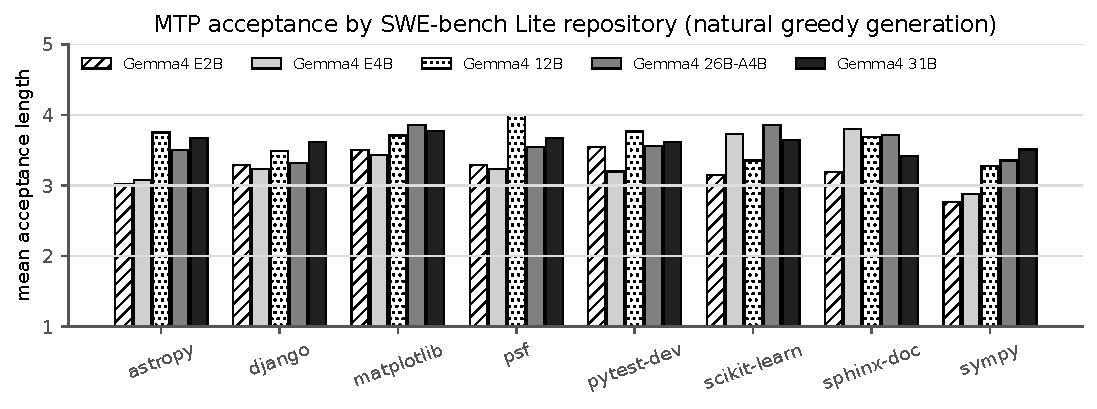
\includegraphics[width=\linewidth]{mtp_swe_genre.pdf}
\caption{SWE-bench Lite のリポジトリ別のmean acceptance length（$\gamma=4$，greedy 生成）．}
\label{fig:genre}
\end{figure}
\begin{figure}[htbp]\centering
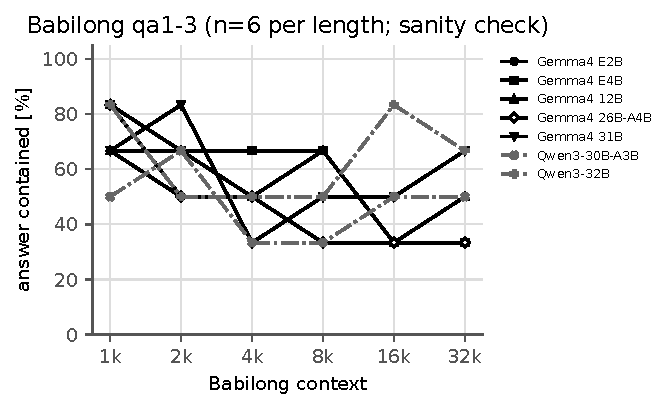
\includegraphics[width=0.6\linewidth]{babilong_accuracy.pdf}
\caption{Babilong qa1--qa3 の正答率（出力冒頭 80 文字に正解語を含む割合，各長さ 6 件）．
性能計測の健全性チェックであり，件数が少ないため精度の比較には使えない．}
\end{figure}


\begin{thebibliography}{99}
\bibitem{gemma4tr} Gemma Team, Google DeepMind. \textit{Gemma 4 Technical Report}, 2026.
\bibitem{gemma4card} Google. \textit{Gemma 4 model card}. \url{https://ai.google.dev/gemma/docs/core/model_card_4}
\bibitem{hfblog} Hugging Face. \textit{Welcome Gemma 4: Frontier multimodal intelligence on device}, 2026. \url{https://huggingface.co/blog/gemma4}
\bibitem{gemma4x} @googlegemma, X, 2026-05-05. \url{https://x.com/googlegemma/status/2051694045869879749}
\bibitem{mtpblog} Google. \textit{Multi-token prediction in Gemma 4}. \url{https://blog.google/innovation-and-ai/technology/developers-tools/multi-token-prediction-gemma-4/}
\bibitem{vllmpr} vLLM PR \#41745, \textit{[Spec Decode] Add Gemma4 MTP speculative decoding support}. \url{https://github.com/vllm-project/vllm/pull/41745}
\bibitem{kipply} kipply. \textit{Transformer Inference Arithmetic}, 2022. \url{https://kipp.ly/transformer-inference-arithmetic/}
\bibitem{kotoba} Kotoba Technologies. \textit{LLM Serving を支える技術}. \url{https://zenn.dev/kotoba_tech/articles/98feb05f24c082}
\bibitem{babilong} Kuratov et al. \textit{BABILong}. \url{https://huggingface.co/datasets/RMT-team/babilong}
\bibitem{swebench} Jimenez et al. \textit{SWE-bench}. \url{https://huggingface.co/datasets/SWE-bench/SWE-bench_Lite}
\bibitem{h100} NVIDIA. \textit{H100 Tensor Core GPU Datasheet}.
\bibitem{jarvislabs} JarvisLabs. \textit{Benchmarking Gemma 4 MTP vs DFlash on a Single H100}. \url{https://jarvislabs.ai/blog/gemma-4-mtp-vs-dflash-benchmark}
\bibitem{inferencebench} InferenceBench. \textit{Gemma 4 31B on H100: The Complete Inference Benchmark}. \url{https://inferencebench.io/blog/gemma-4-31b-h100-complete-inference-benchmark/}
\bibitem{vllmissue38887} vLLM Issue \#38887, \textit{Gemma 4 E4B extremely slow on v0.19.0: forced TRITON\_ATTN fallback}. \url{https://github.com/vllm-project/vllm/issues/38887}
\bibitem{vllmpr38891} vLLM PR \#38891, \textit{[Gemma4] Allow per-layer attention backend selection for heterogeneous head dimensions}. \url{https://github.com/vllm-project/vllm/pull/38891}
\bibitem{h100wp} NVIDIA. \textit{NVIDIA H100 Tensor Core GPU Architecture} (whitepaper), 2022.
\bibitem{nvperf} NVIDIA. \textit{GPU Performance Background User's Guide}. \url{https://docs.nvidia.com/deeplearning/performance/dl-performance-gpu-background/index.html}
\bibitem{cudaguide} NVIDIA. \textit{CUDA C++ Programming Guide}. \url{https://docs.nvidia.com/cuda/cuda-c-programming-guide/}
\bibitem{volkov} V. Volkov. \textit{Understanding Latency Hiding on GPUs}. PhD thesis, UC Berkeley, Technical Report UCB/EECS-2016-143, 2016.
\bibitem{palm} A. Chowdhery et al. \textit{PaLM: Scaling Language Modeling with Pathways}. arXiv:2204.02311, 2022.
\end{thebibliography}
\end{document}
